% THIS IS CURRENTLY A ROUGH DRAFT
% QUESTION: How do I deal with experiment repeats?  Do I pile the data together, or do I put them in the appendix?
% TODO:
% - Bullet points -> prose
% - Notes/random ideas jotted down -> comments

\chapter{Microfluidics and fluorescence microscopy for cellular metabolic cycles}
\label{ch:biology}

There is a paucity of studies of the yeast metabolic cycle at the cellular level --- i.e.\ in which budding yeast cells are investigated in isolation rather than as a population.
Previous population-level studies in the chemostat, by their very nature, fail to account for cell-to-cell heterogeneity and create cell density and environmental conditions that are far removed from the natural habitat of budding yeast.

Here, I use single-cell microfluidics to physically separate budding yeast cells and use fluorescence microscopy to monitor the yeast metabolic cycle and the cell division cycle.
I do so in order to address the relationship between the metabolic and cell division cycle, and whether nutrient and genetic perturbations affect the metabolic cycle as was previously reported in chemostat-based studies.
Specifically, I culture wild-type and engineered strains, including deletion strains, in microfluidic chambers that force the cells to physically separate.
Each cell in a trap is monitored while it undergoes growth and cell division: brightfield images and images of flavin fluorescence are taken.
In some experiments, I use the microfluidics set-up to create rapid changes in the nutrient medium at specified times to assess the cells' response.

My aims in this chapter are:
\begin{enumerate}
  \item To confirm that flavin autofluorescence can be used to monitor the yeast metabolic cycle \parencite{baumgartnerFlavinbasedMetabolicCycles2018}, and to confirm autonomy of the metabolic oscillator from the cell division oscillator.
  \item To show the robustness of the yeast metabolic cycle across nutrient conditions and deletion strains.
  \item To address whether observations of the behaviour of the metabolic cycles of deletion strains in the chemostat can be recapitulated in single-cell conditions.
        And, if behaviours differ, offer an explanation based on cell-to-cell heterogeneity.
\end{enumerate}

\section[Permissive conditions]{Single-cell flavin oscillations synchronise with cell division cycle in permissive conditions.}
\label{sec:biology-sync}

\begin{figure}
  \centering
    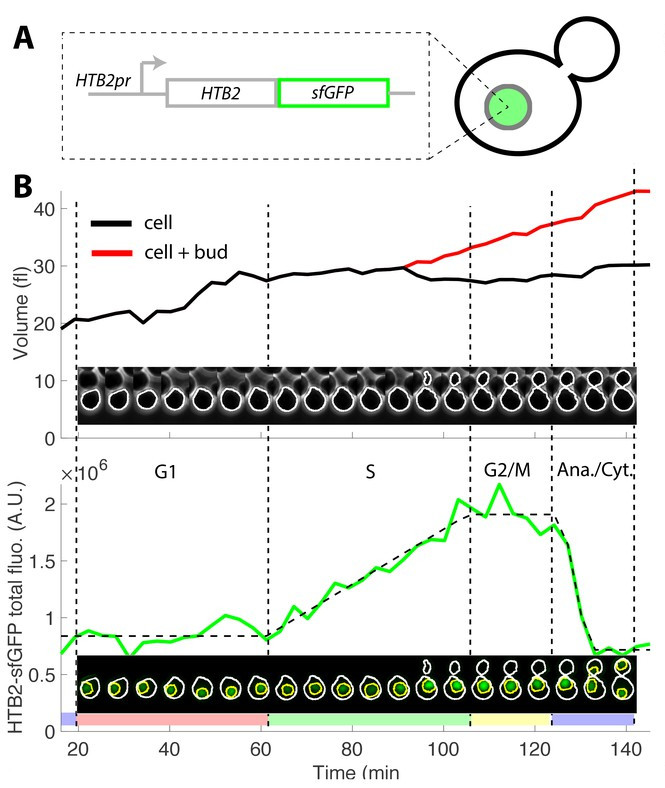
\includegraphics[width=0.5\linewidth]{garmendia-torresMultipleInputsEnsure2018_1_adapted.jpg}
    \caption{
      Engineering a fluorescent protein cassette fused to \textit{HTB2} (A) allows the identification of phases of the cell division cycle by modelling the fluorescent protein intensity changes over time as piecewise linear sections (B).
      Adapted from \textcite{garmendia-torresMultipleInputsEnsure2018}.
    }
  \label{fig:biology-htb2}
\end{figure}

To replicate the single-cell flavin oscillations observed by \textcite{baumgartnerFlavinbasedMetabolicCycles2018}, I cultured FY4 HTB2::mCherry cells in minimal medium supplemented with \SI{20}{\gram~\litre^{-1}} glucose, over \SI{24}{\hour} in the microfluidic device.
These cells are prototrophic, owing to its FY4 background, allowing me to rule out the effects of certain nutrient supplements on the metabolic cycle.
I engineered an insertion to the \textit{HTB2} gene to attach a fluorescent protein to histone 2B so that imaging of the fluorescence protein shows phases of the cell division cycle, as performed by ~\textcite{garmendia-torresMultipleInputsEnsure2018} (figure~\ref{fig:biology-htb2}).
I chose mCherry as the fluorescent protein because the GFP emission spectrum overlaps with the flavin emission spectrum, and because mutual information does not show a significant difference between GFP and superfolder GFP traces (figure ...).
Finally, I chose the high glucose concentration \SI{20}{\gram~\litre^{-1}} glucose as it is commonly used as a permissive growth condition for budding yeast cultivation experiments.

Replicating a previous flavin-based microfluidics study to confirm that my experimental set-up monitors the yeast metabolic cycle is important.
This is because I use a different single-cell microfluidics setup from previous studies and we use flavin, a fluorescent compound that is less used as an indicator of the yeast metabolic cycle.
In addition, I aim to show the use of a more informative cell division cycle marker, compared to the more commonly used Whi5p, along with automated identification of budding events using \textit{BABY} \parencite{pietschDeterminingGrowthRates2023}.


\begin{figure}
  \centering
    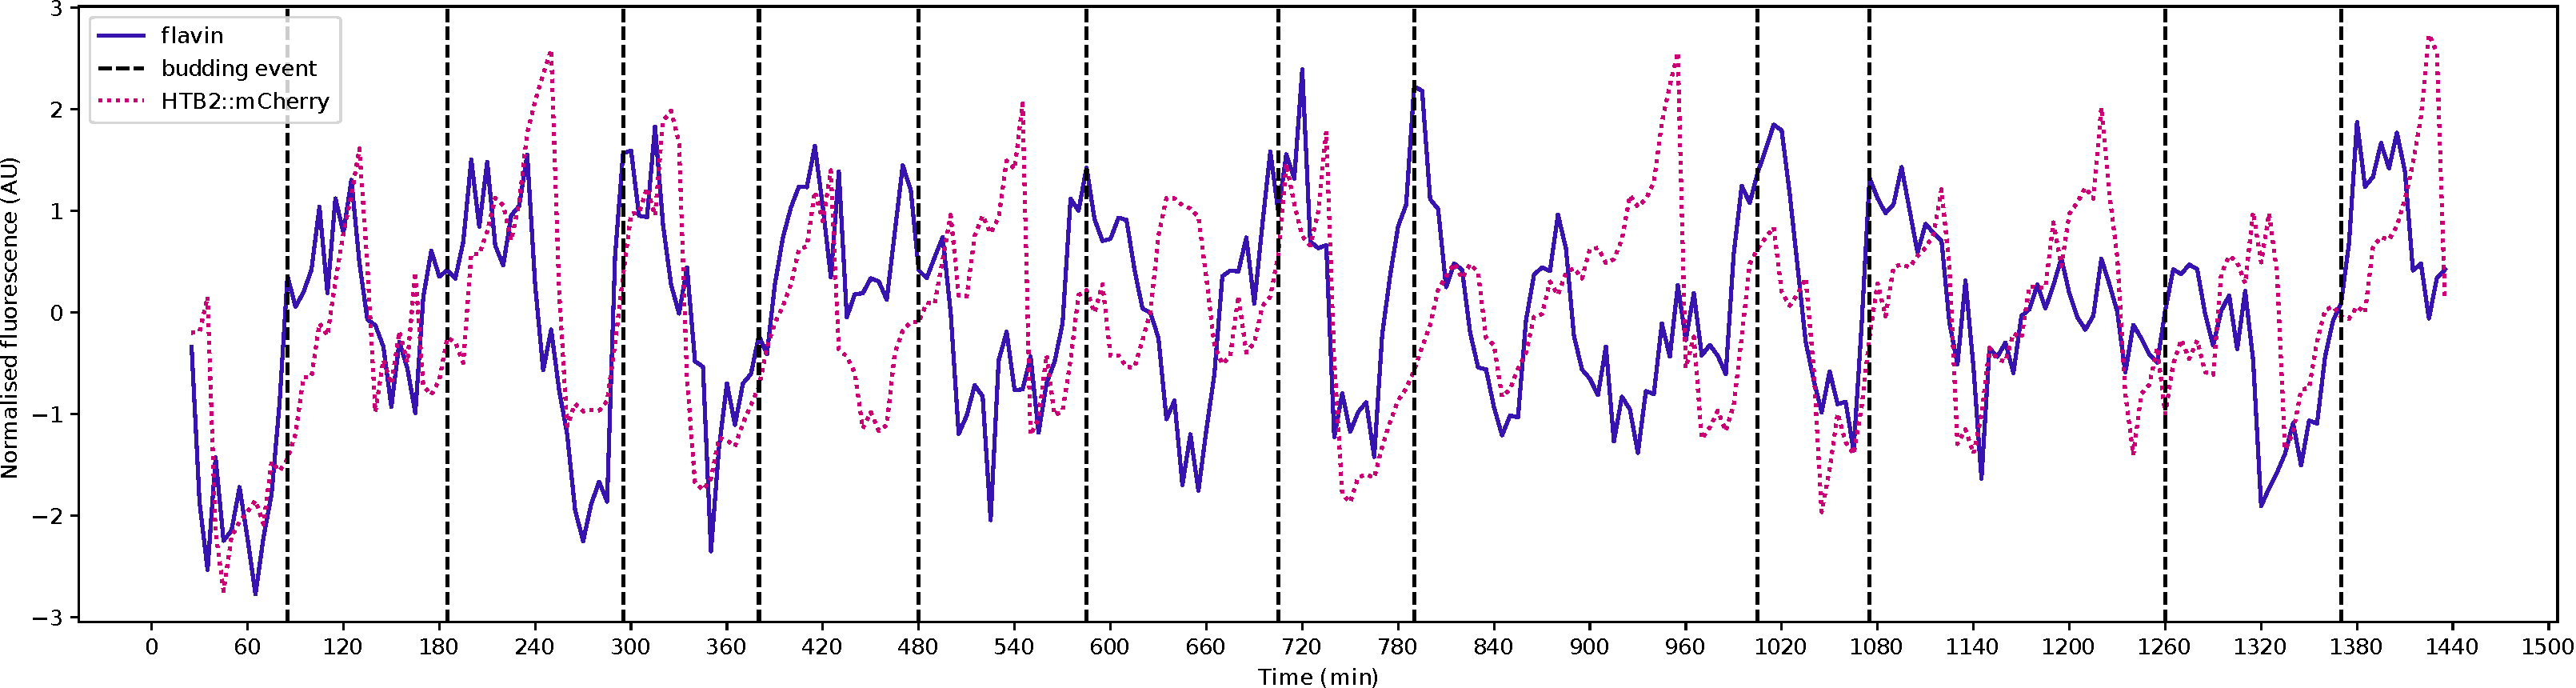
\includegraphics[width=1.0\linewidth]{single_birth_plot_edit.pdf}
    \caption{
      Oscillations of flavin fluorescence in the yeast metabolic cycle synchronise with events in the cell division cycle.
      Figure shows sample flavin fluorescence (purple, solid lines) and histone 2B (pink, dotted lines) level in a single FY4 HTB2::mCherry cell grown in \SI{20}{\gram~\litre^{-1}} glucose.
      Vertical lines (black, dashed) indicate budding.
    }
  \label{fig:biology-highglc-single}
\end{figure}

In this experiment, I observed oscillations in the fluorescence of flavins over time from single cells (figure~\ref{fig:biology-highglc-single}).
For a given cell, these oscillations peak when a bud forms, approximately during G2/M.
This relationship between flavin oscillations and the cell division cycle indeed agrees with \textcite{baumgartnerFlavinbasedMetabolicCycles2018}.
I expect the flavin fluorescence to peak when buds form, and this is my reasoning:
NAD(P)H fluorescence peaks --- i.e. the molecule is in the reduced NAD(P)H form --- when buds form \parencite{papagiannakisAutonomousMetabolicOscillations2017}.
Flavins should be in the oxidised form when NAD(P)H is in the reduced form because the flavoprotein lipoamide dehydrogenase is in redox equilibrium with NAD(P)H \parencite{sianoNADHFlavinFluorescence1989}.
Flavins fluoresce in the oxidised form, thus we expect flavin fluorescence to peak.
Furthermore, \textcite{murrayRedoxRegulationRespiring2011} confirms that flavin and NAD(P)H fluorescence peak at the same time in continuous chemostat cultures.

There were some cases in which there was an oscillation without cell division cycle progression or bud formation (figure ...).
Such cases, also revealed by \textcite{papagiannakisAutonomousMetabolicOscillations2017} via NAD(P)H cycles, confirm that the metabolic cycle is generated autonomously from the cell division cycle.


\begin{figure}
  \centering
  \begin{subfigure}[htpb]{0.4\textwidth}
   \centering
   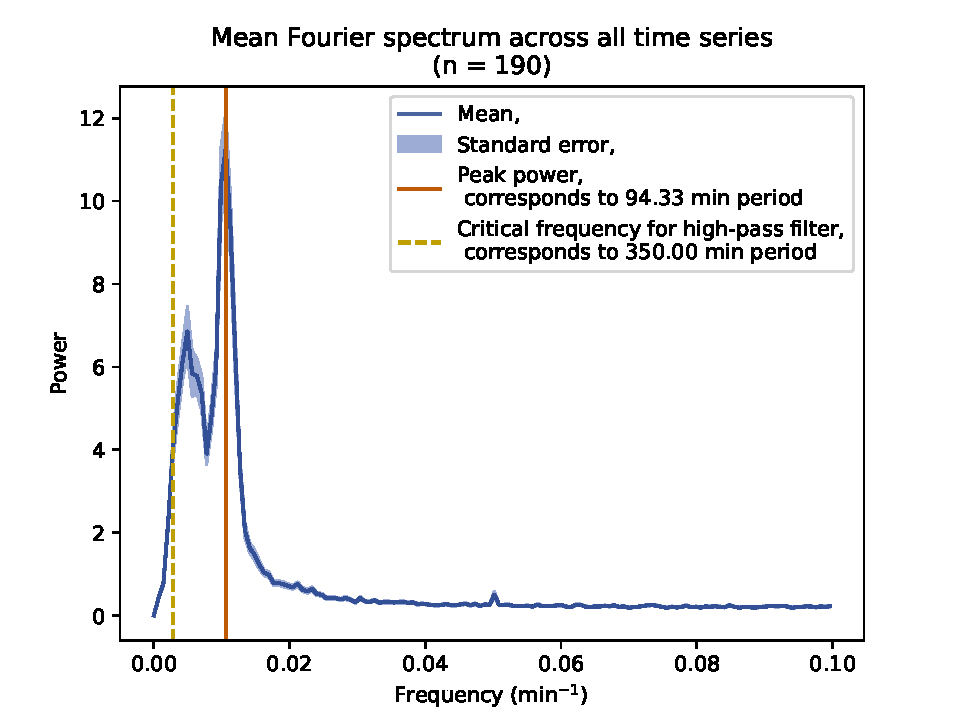
\includegraphics[width=\textwidth]{htb2mCherry_26643_14}
   \caption{
    Mean Fourier spectrum of flavin fluorescence across cells.
   }
   \label{fig:biology-highglc-sync-fourier}
  \end{subfigure}%
  \begin{subfigure}[htpb]{0.4\textwidth}
   \centering
   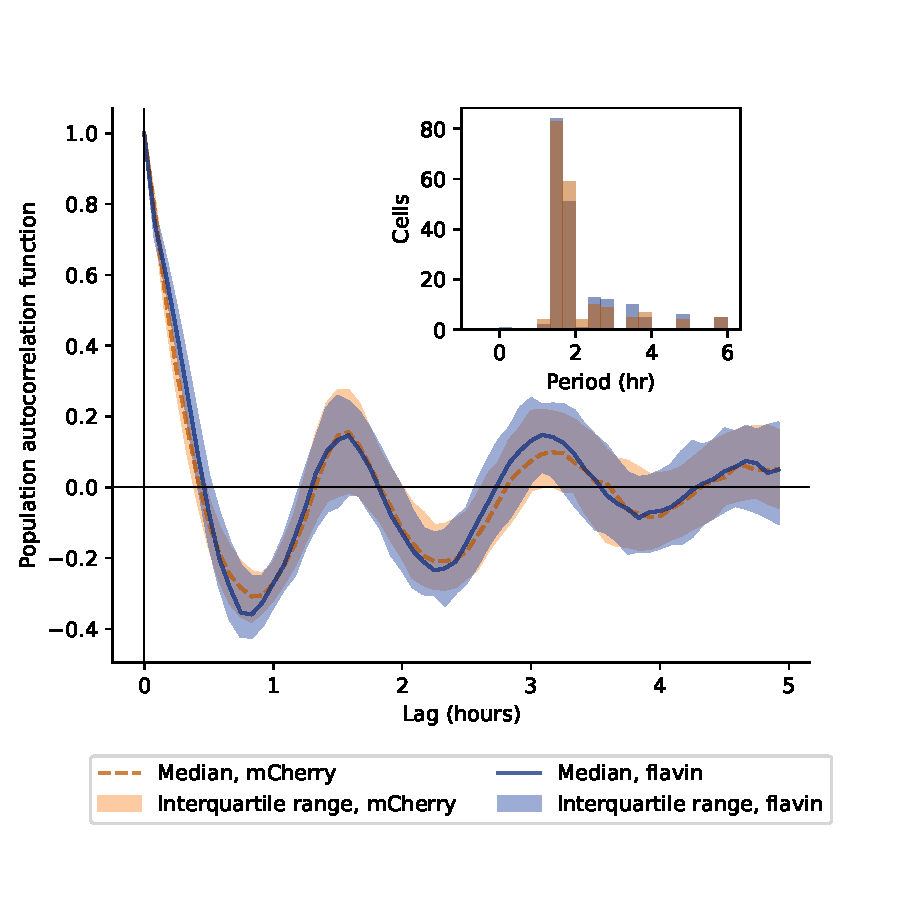
\includegraphics[width=\textwidth]{htb2mCherry_26643_12}
   \caption{
     \textbf{(Main)} Median autocorrelation functions of flavin fluorescence (blue) and histone 2B levels (orange) time series,
     along with \textbf{(inset)} the periods of each oscillator across cells as determined by the strongest frequency in each signal's Fourier spectrum.
   }
   \label{fig:biology-highglc-sync-acf}
  \end{subfigure}

  \begin{subfigure}[htpb]{0.4\textwidth}
   \centering
   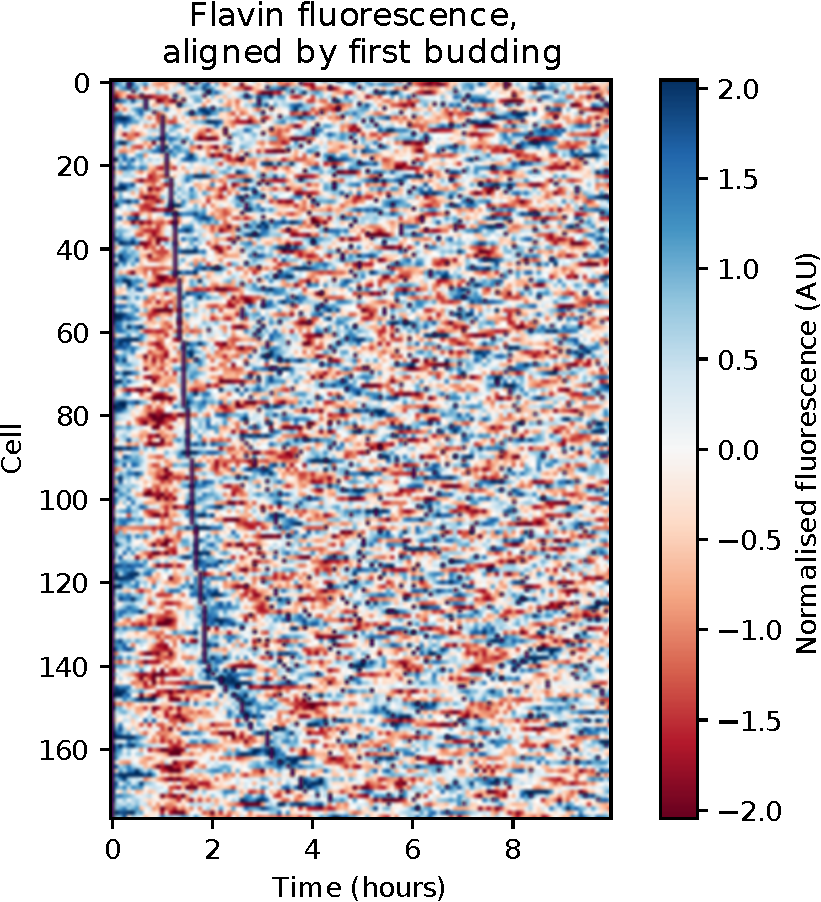
\includegraphics[width=\textwidth]{heatmap_edit.pdf}
   \caption{
     Heatmap shows the flavin fluorescence (pixels on a red-blue scale) and budding events (black pixels) of each cell.
     Signals are aligned by the first budding event.
   }
   \label{fig:biology-highglc-sync-heatmap}
  \end{subfigure}%
  \begin{subfigure}[htpb]{0.4\textwidth}
   \centering
   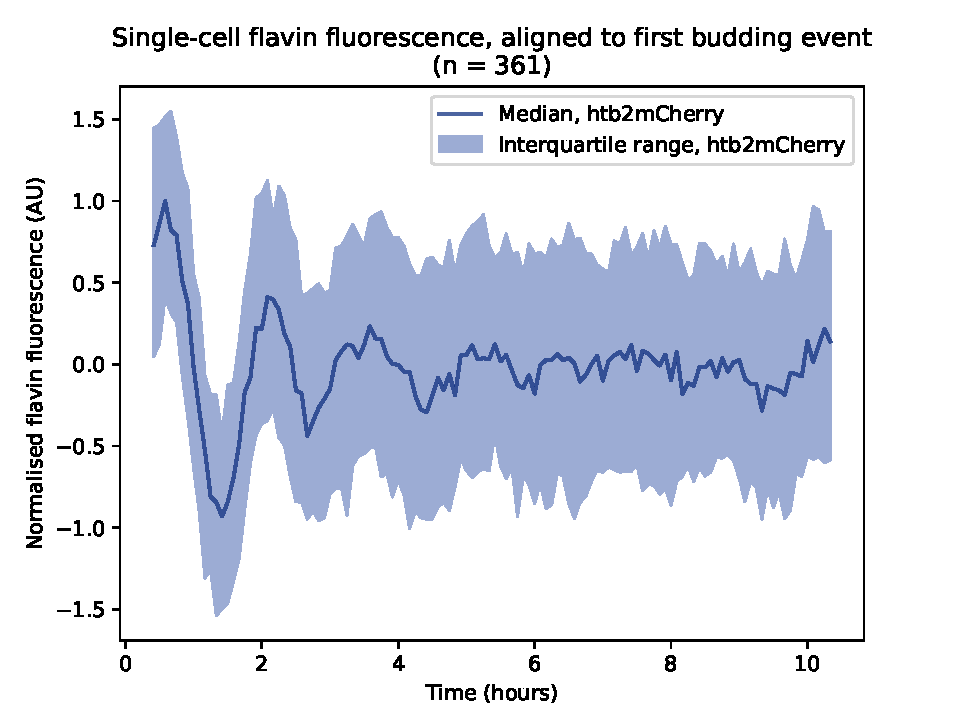
\includegraphics[width=\textwidth]{htb2mCherry_26643_6}
   \caption{
    Median flavin fluorescence signal across cells, aligned to first budding event.
   }
   \label{fig:biology-highglc-sync-median}
  \end{subfigure}

  \begin{subfigure}[htpb]{0.4\textwidth}
   \centering
   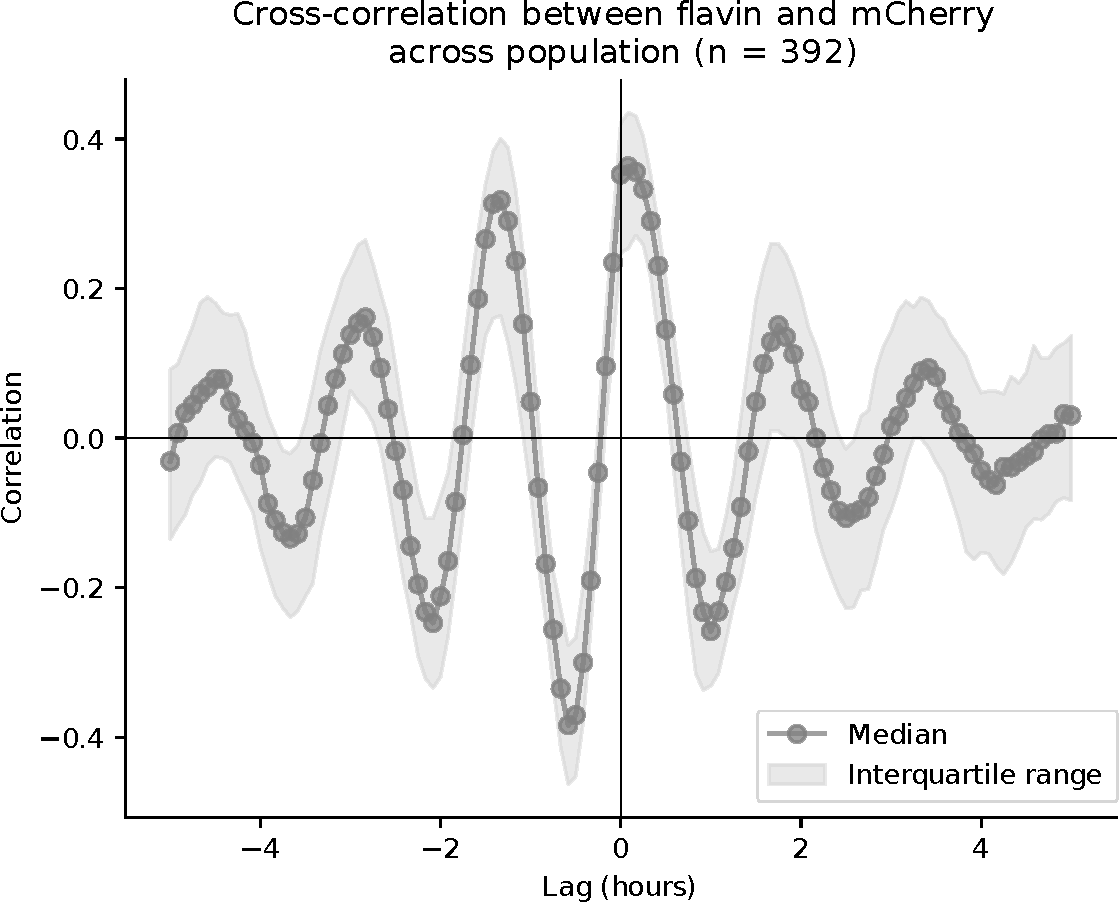
\includegraphics[width=\textwidth]{xcf_edit.pdf}
   \caption{
    Cross-correlation between flavin and histone 2B signals.
   }
   \label{fig:biology-highglc-sync-xcf}
  \end{subfigure}

  \caption{
    The yeast metabolic cycle and cell division cycle synchronise within each cell in a population of FY4 HTB2::mCherry cells under the same conditions (\SI{20}{\gram~\litre^{-1}} glucose).
  }
  \label{fig:biology-highglc-sync}
\end{figure}

% TODO: Add references to chapter 3 re the analysis methods
To quantify the period of the oscillators, I used several methods that confirm each other.
First, I computed the Fourier spectrum of each flavin time series, originating from each cell.
Only time series that had data points that filled all time points in the experiment were used, as the Fourier spectrum can only be calculated for such time series.
The mean of these spectra across each time series was computed (figure~\ref{fig:biology-highglc-sync-fourier}), and the peak power suggests a \SI{94.33}{\minute} period of the metabolic oscillations.
In addition, the peak power from the Fourier spectrum of each cell was determined and the distribution of such peaks was shown in a histogram to show the distribution of the periods across the population (figure~\ref{fig:biology-highglc-sync-acf} inset), additionally confirming a $\approx$\SI{90}{\minute} period.
This computation was also repeated for the mCherry time series.
Second, I computed the autocorrelation function of flavin time series and of mCherry time series across the population of cells, confirming a $\approx$\SI{90}{\minute} period for both time series (figure~\ref{fig:biology-highglc-sync-acf}).
% [CITATIONS NEEDED]
Taken together, these methods suggest that both the metabolic and cell division cycle of the prototrophic strain in high-glucose conditions occur at a period of approximately \SI{90}{\minute}, which agrees with the literature regarding the duration of the cell division cycle in such permissive growth conditions.

To visualise the relationship between the metabolic cycle and the cell division cycle, I showed the flavin fluorescence and budding events in a heatmap.
In figure~\ref{fig:biology-highglc-sync-heatmap},
each row of pixels represents a cell.
Fluorescence is represented as colours (red-blue), with red indicating low signal and blue indicating high signal.
Each budding event is indicated as a black pixel.
Signals are aligned by the first budding event to show that
(a) budding events synchronise with peaks in fluorescence, and
(b) the cell division cycle varies between cells.
The heatmap shows that most first cell division cycles --- shown as the first interval between budding events --- are just under \SI{2}{\hour}, with cell-to-cell variations, agreeing with figure~\ref{fig:biology-highglc-sync-acf} (inset).
It also shows that the budding events coincide with peaks in flavin fluorescence.
Additionally, the median of the flavin signals aligned by the first birth event is computed (figure~\ref{fig:biology-highglc-sync-median}), and the oscillatory shape of the median confirms the synchrony between the metabolic cycle and budding events.

To quantify the relationship between the metabolic cycle and the cell division cycle, I computed the cross-correlation function between the flavin and mCherry signals across the population (figure~\ref{fig:biology-highglc-sync-xcf}).
This function shows that the mCherry signals are, on average, shifted by \SI{5}{\minute} relative to the flavin signals.

Figure~\ref{fig:biology-highglc-sync} thus confirms that, consistently across a population of physically separated prototrophic cells, the metabolic cycle and the cell division cycle synchronise, with flavin intensity peaking as the cell forms a bud in G2/M phase.


% Figure & discussion of BY4741.
\begin{figure}
  \centering
  \begin{subfigure}[htpb]{0.4\textwidth}
   \centering
   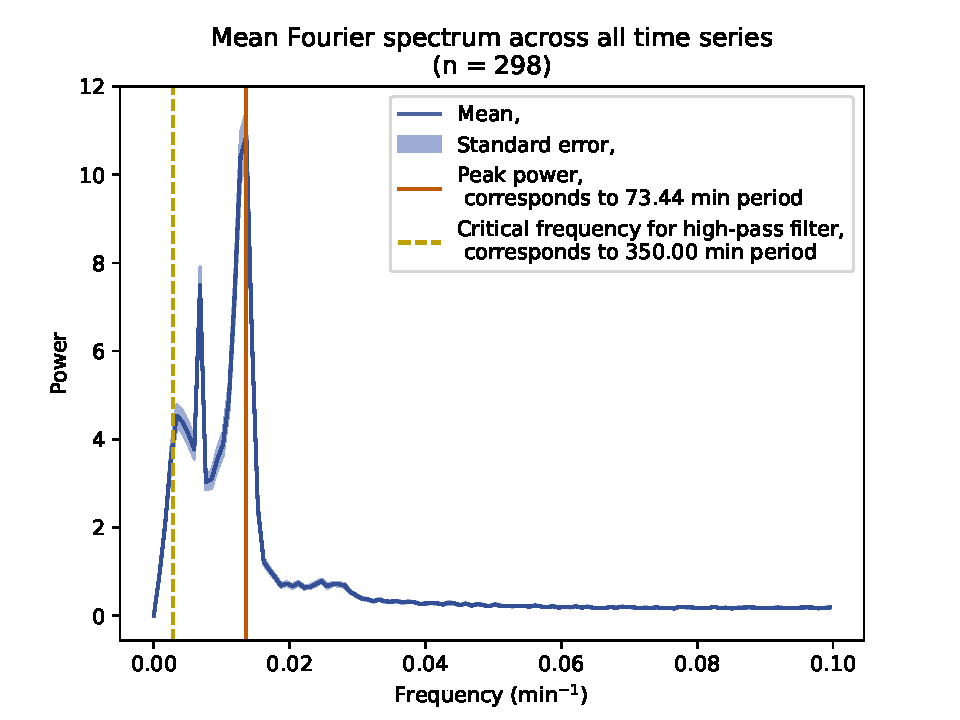
\includegraphics[width=\textwidth]{by4741_491_13}
   \caption{
    Mean Fourier spectrum of flavin fluorescence across cells.
   }
   \label{fig:biology-by4741-sync-fourier}
  \end{subfigure}%
  \begin{subfigure}[htpb]{0.4\textwidth}
   \centering
   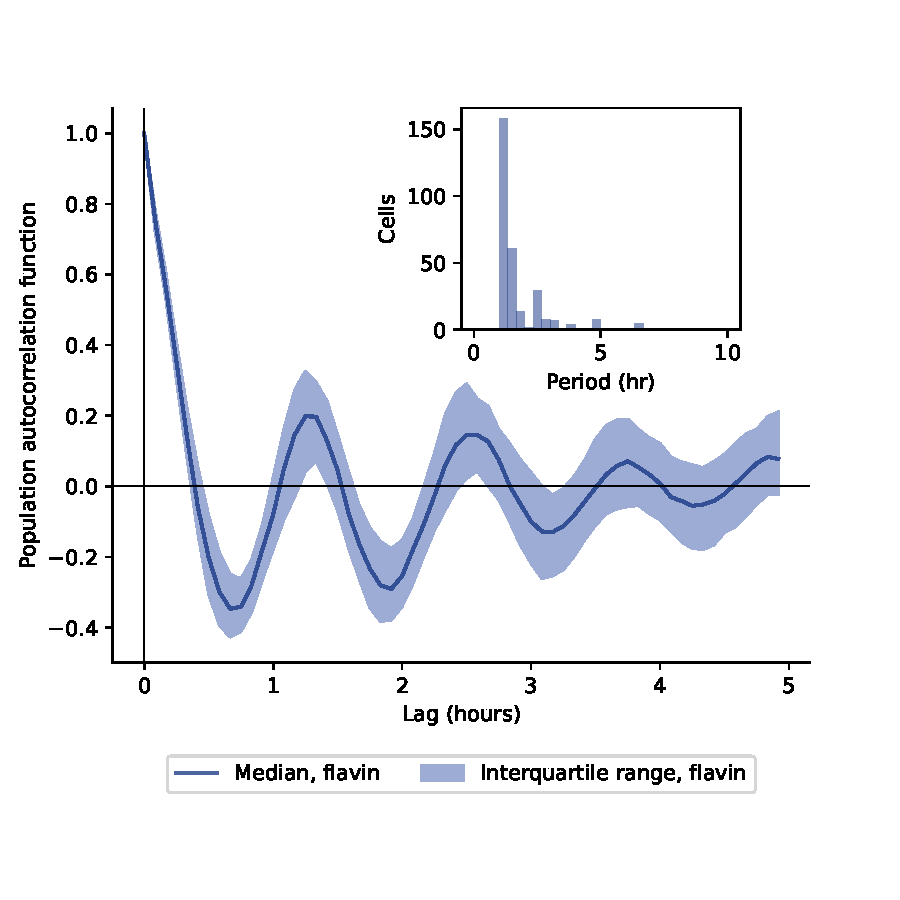
\includegraphics[width=\textwidth]{by4741_491_12}
   \caption{
     \textbf{(Main)} Median autocorrelation function flavin fluorescence,
     along with \textbf{(inset)} the periods across cells as determined by the strongest frequency in each signal's Fourier spectrum.
   }
   \label{fig:biology-by4741-sync-acf}
  \end{subfigure}

  \begin{subfigure}[htpb]{0.4\textwidth}
   \centering
   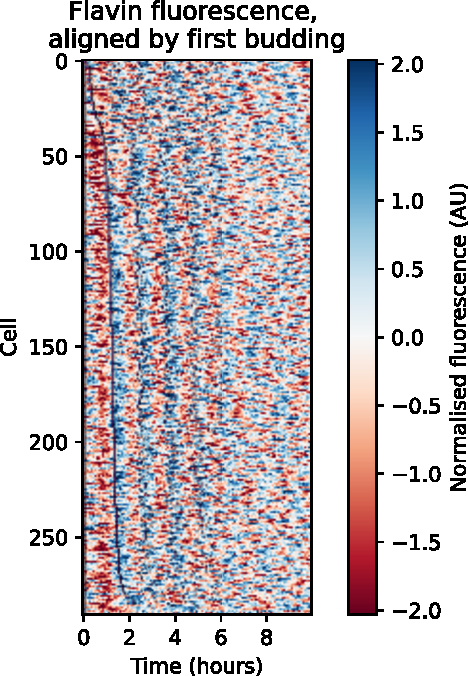
\includegraphics[width=\textwidth]{by4741_491_7.pdf}
   \caption{
    Heatmap shows the flavin fluorescence of each cell in a population over time.
    Each budding event is indicated as a black pixel.
    Signals are aligned by the first budding event.
   }
   \label{fig:biology-by4741-sync-heatmap}
  \end{subfigure}%
  \begin{subfigure}[htpb]{0.4\textwidth}
   \centering
   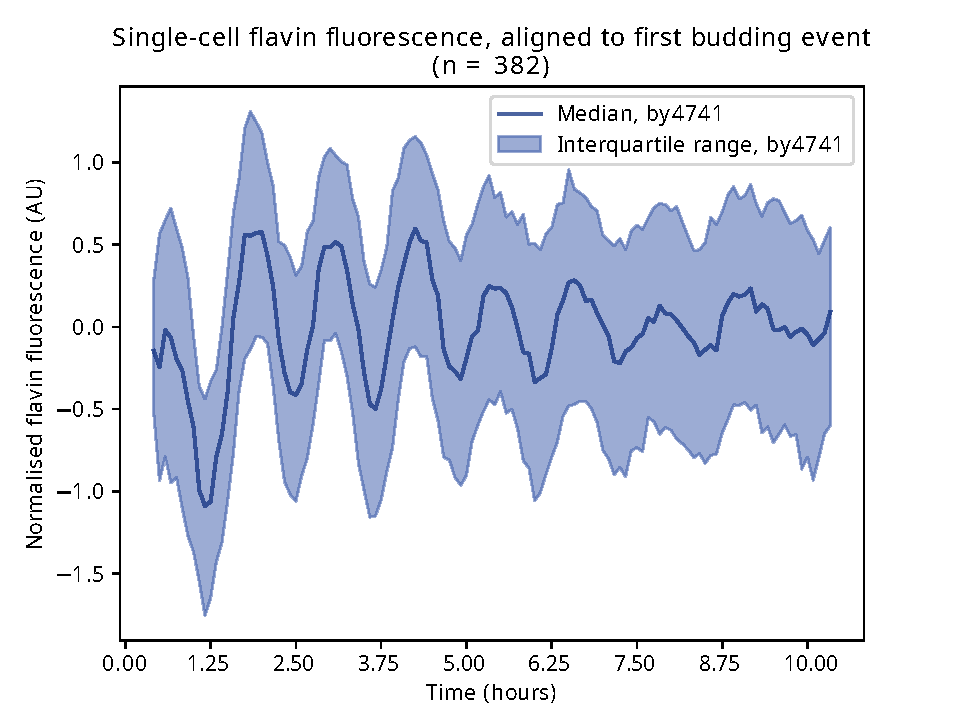
\includegraphics[width=\textwidth]{by4741_491_6}
   \caption{
    Median flavin fluorescence signal across cells.
   }
   \label{fig:biology-by4741-sync-median}
  \end{subfigure}

  \caption{
    Cells of the BY4741 strain consistently show an approximately 75-hour cycle of flavin oscillations.
    The presence of such oscillations in an auxotrophic strain highlights the robustness of the yeast metabolic cycle.
  }
  \label{fig:biology-by4741-sync}
\end{figure}

To show that the metabolic cycle is robust, I performed a similar experiment on an auxotrophic strain, which has genetic mutations that make it unable to grow in media lacking certain nutrients.
I cultured BY4741 cells in minimal medium supplemented with uracil and the amino acids required for this strain to grow, plus \SI{10}{\gram~\litre^{-1}} glucose.
Showing that metabolic cycles occur in an auxotroph is important because it confirms that the YMC is robust --- a lot of things must be impaired for the cycle to disappear --- and thus likely an intrinsic cycle of budding yeast.
Similar to FY4 HTB2::mCherry cells, BY4741 cells show robust, consistent oscillations in flavin fluorescence that peak upon budding (figure~\ref{fig:biology-by4741-sync}), although metabolic cycles have a period of $\approx$\SI{75}{\minute} in this case.
The shorter period, implying a higher growth rate, may be explained by a lack of burden caused by a lack of an mCherry insertion, and by media supplements.
% Discussion (probably in discussion section at the end): to be 'proper', I should perform an experiment with the BY4741 HTB2::mCherry I engineered.


\section[Abrupt nutrient changes]{Cells autonomously generate flavin oscillations, independently of the cell division cycle, in response to abrupt nutrient changes.}
\label{sec:biology-abrupt}

To provide additional evidence that cells generate metabolic oscillations independent of the cell division cycle, I created a condition in which cells do not undergo cell division.
Previously, \textcite{baumgartnerFlavinbasedMetabolicCycles2018} did so by treating cells with the cell division cycle inhibitor rapamycin, while \textcite{papagiannakisAutonomousMetabolicOscillations2017} treated cells with the mating pheromone alpha factor to induce arrest in G1.
In contrast, I halt cell division cycles by changing nutrient conditions.
Specifically, I take advantage of fast-switching in ALCATRAS by inducing abrupt starvation, similar to experiments described by \textcite{bagameryPutativeBetHedgingStrategy2020} that investigated the heterogeneity of cellular responses to starvation.
In addition, such a starvation study would shed light to whether a diffusible metabolite is responsible for the synchrony of the metabolic cycle across cells, as suggested by some chemostat-based and modelling studies. % CITATION NEEDED -- consult introduction.

\begin{figure}
  \centering
  \begin{subfigure}[htpb]{1.0\textwidth}
   \centering
   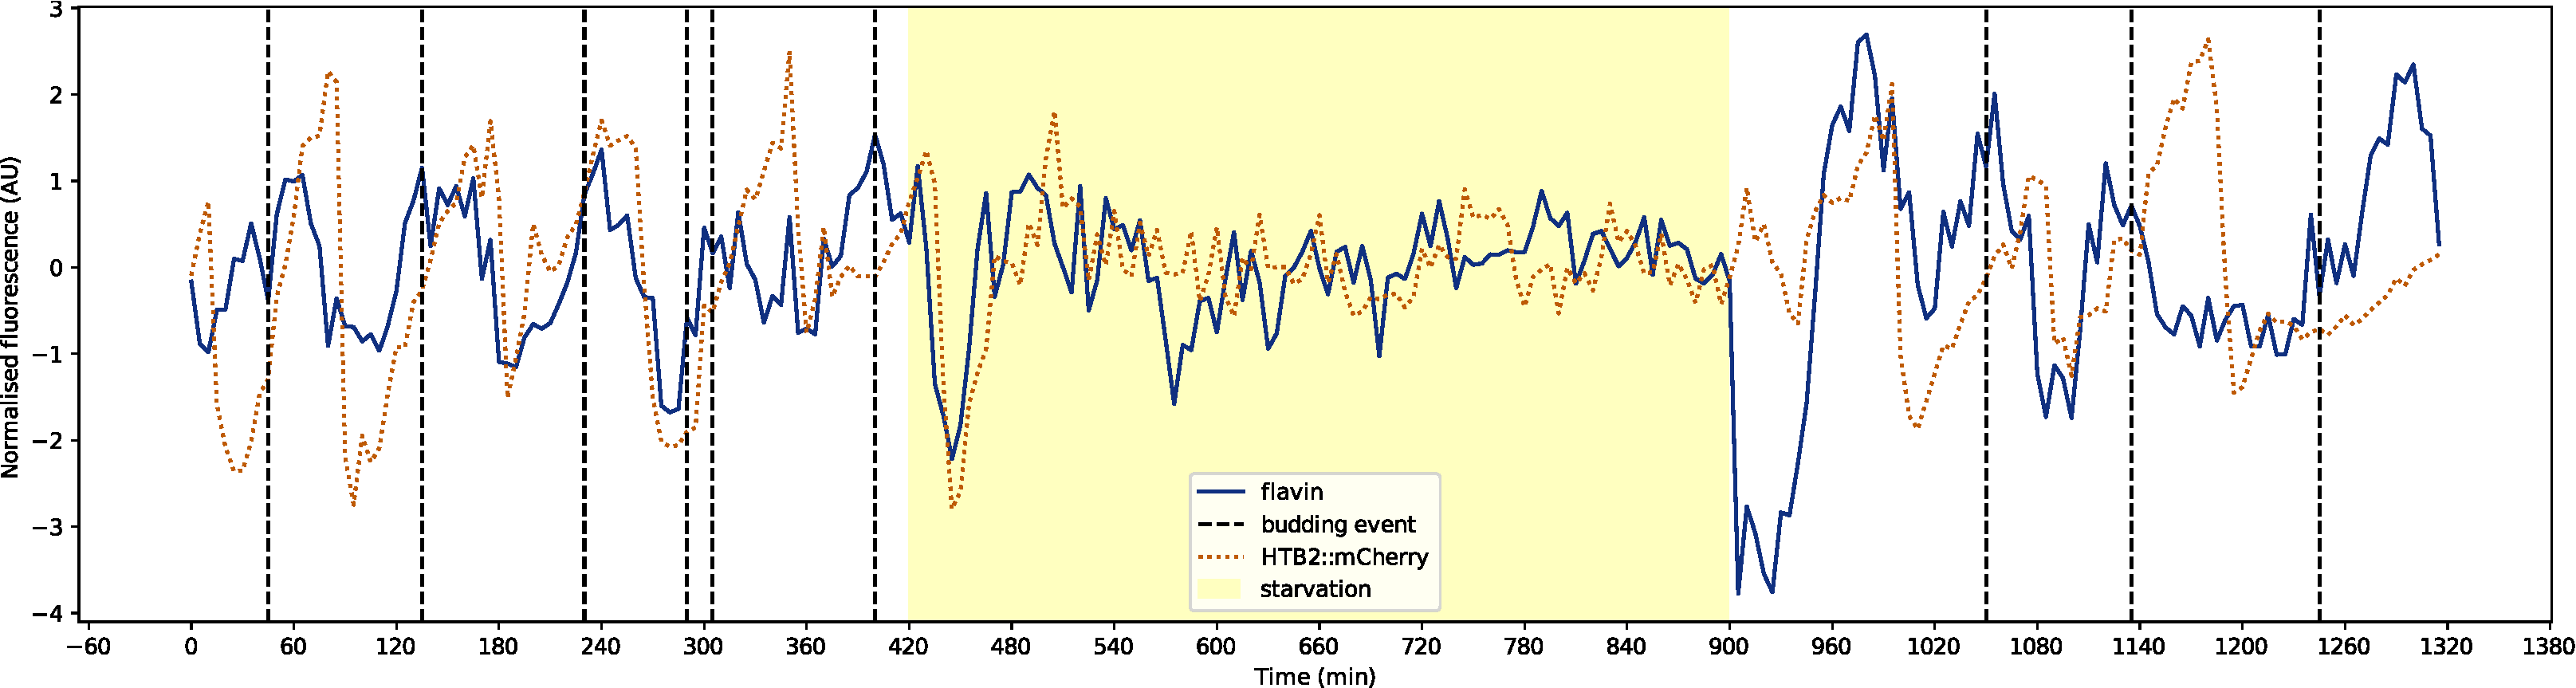
\includegraphics[width=\textwidth]{starvation_single_birth_plot_new_edit.pdf}
   \caption{
     Flavin fluorescence synchronises with the cell division cycle in high-glucose conditions before and after starvation (FY4 HTB2::mCherry).
     %Figure shows sample flavin fluorescence levels (purple) and histone 2B localisation (pink) in single cells.
     %Vertical lines (black) indicate budding.
   }
   \label{fig:biology-starvation-single}
  \end{subfigure}

  \begin{subfigure}[htpb]{0.7\textwidth}
   \centering
   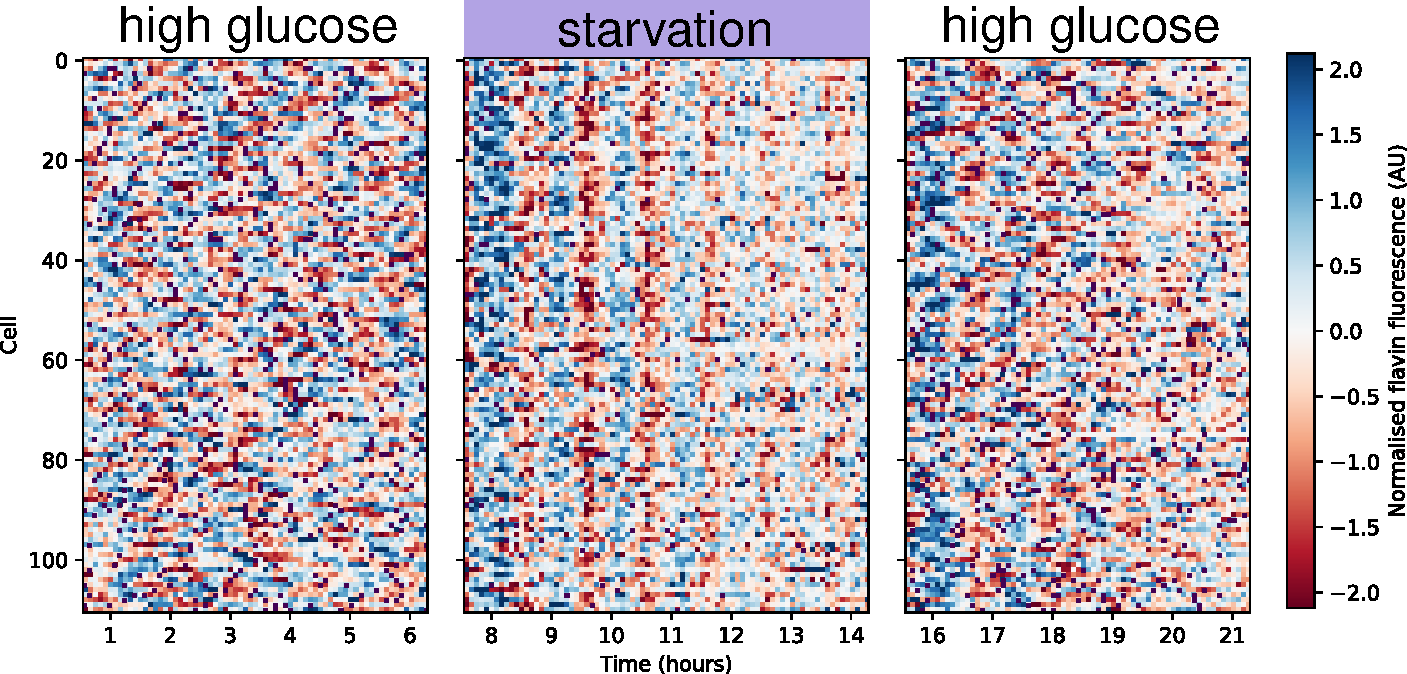
\includegraphics[width=\textwidth]{heatmap_012_edit.pdf}
   \caption{
     Heatmap shows the flavin fluorescence of each cell (FY4) in a population over time.
     %Each row of pixels represents one of 60 cells.
     %Fluorescence is represented as colours with blue indicating low signal and red indicating high signal.
     Each budding event is indicated as a black pixel.
     During starvation, synchronisation of flavin oscillations between cells were observed, and budding events were sparse.
   }
   \label{fig:biology-starvation-heatmap}
  \end{subfigure}

  \caption{
     Metabolic cycles between physically separated cells synchronise upon abrupt starvation.
     FY4 and HTB2::mCherry cells were grown in \SI{7.5}{\gram~\litre^{-1}} glucose for \SI{7}{\hour} before being abruptly switched to \SI{0}{\gram~\litre^{-1}} glucose for \SI{8}{\hour} and then resumed to \SI{7.5}{\gram~\litre^{-1}} glucose for \SI{7}{\hour}.
  }
  \label{fig:biology-starvation}
\end{figure}


\begin{figure}
  \centering
  \begin{subfigure}[htpb]{0.7\textwidth}
   \centering
   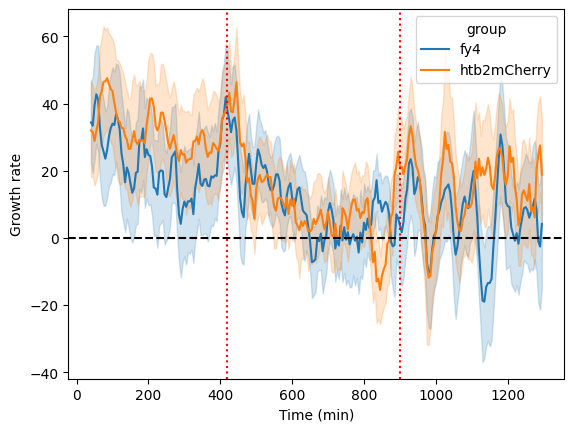
\includegraphics[width=\textwidth]{allstrains_19972_gr}
   \caption{
     Growth rate
   }
   \label{fig:biology-starvation-gr}
  \end{subfigure}

  \begin{subfigure}[htpb]{0.7\textwidth}
   \centering
   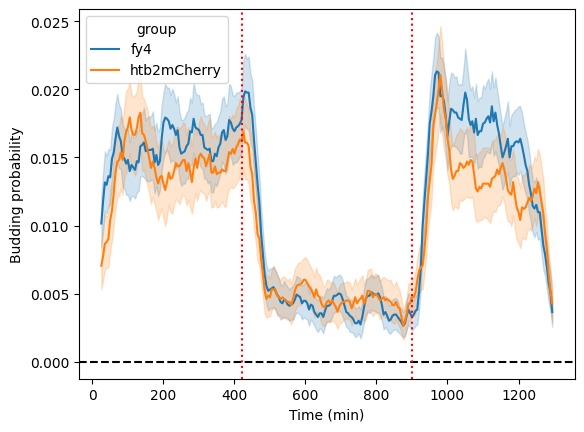
\includegraphics[width=\textwidth]{allstrains_19972_budprob}
   \caption{
     Budding probability
   }
   \label{fig:biology-starvation-budprob}
  \end{subfigure}

  \caption{
    Mean growth rate and budding probability of FY4 (blue) and HTB2::mCherry (orange) strains over time during the glucose-starvation experiment, with 95\% confidence intervals shown (shaded).
    Vertical lines (red) show changes in nutrient media.
  }
  \label{fig:biology-starvation-gr-budprob}
\end{figure}

In this experiment, I cultured FY4 and HTB2::mCherry cells were grown in \SI{7.5}{\gram~\litre^{-1}} glucose for \SI{7}{\hour} before being abruptly switched to \SI{0}{\gram~\litre^{-1}} glucose for \SI{8}{\hour} and then resumed to \SI{7.5}{\gram~\litre^{-1}} glucose for \SI{7}{\hour} (figure~\ref{fig:biology-starvation}).
When cells are in high glucose, oscillations are asynchronous, consistent with section~\ref{sec:biology-sync}, \textcite{papagiannakisAutonomousMetabolicOscillations2017} and \textcite{baumgartnerFlavinbasedMetabolicCycles2018}.
I found that when cells grown in high glucose were abruptly starved of glucose, their flavin oscillations reset phase (figure~\ref{fig:biology-starvation-heatmap}).
These flavin oscillations under starvation continue, while growth rate drops and budding events are sparse (figure~\ref{fig:biology-starvation-gr-budprob}).

The results show that metabolic oscillations may be generated when cell division cycle is halted, providing strong evidence that the metabolic cycle is generated autonomously and independently of the cell division cycle.
In addition, the results show that each cell can individually reset the phase of its metabolic cycle in response to abrupt changes in environmental conditions; similar phenomena have been observed upon bulk addition of carbon sources.
Importantly, the results suggest that diffusion of signalling chemicals between cells is not required for generation of metabolic cycles.
Combined with results from the previous section, my results give weight to the idea that the metabolic cycle responds to external conditions and create windows of opportunity for `firing' the cell division cycle that the cell can choose to not take if conditions are not favourable.


\begin{figure}
  \centering
  \begin{subfigure}[htpb]{1.0\textwidth}
   \centering
   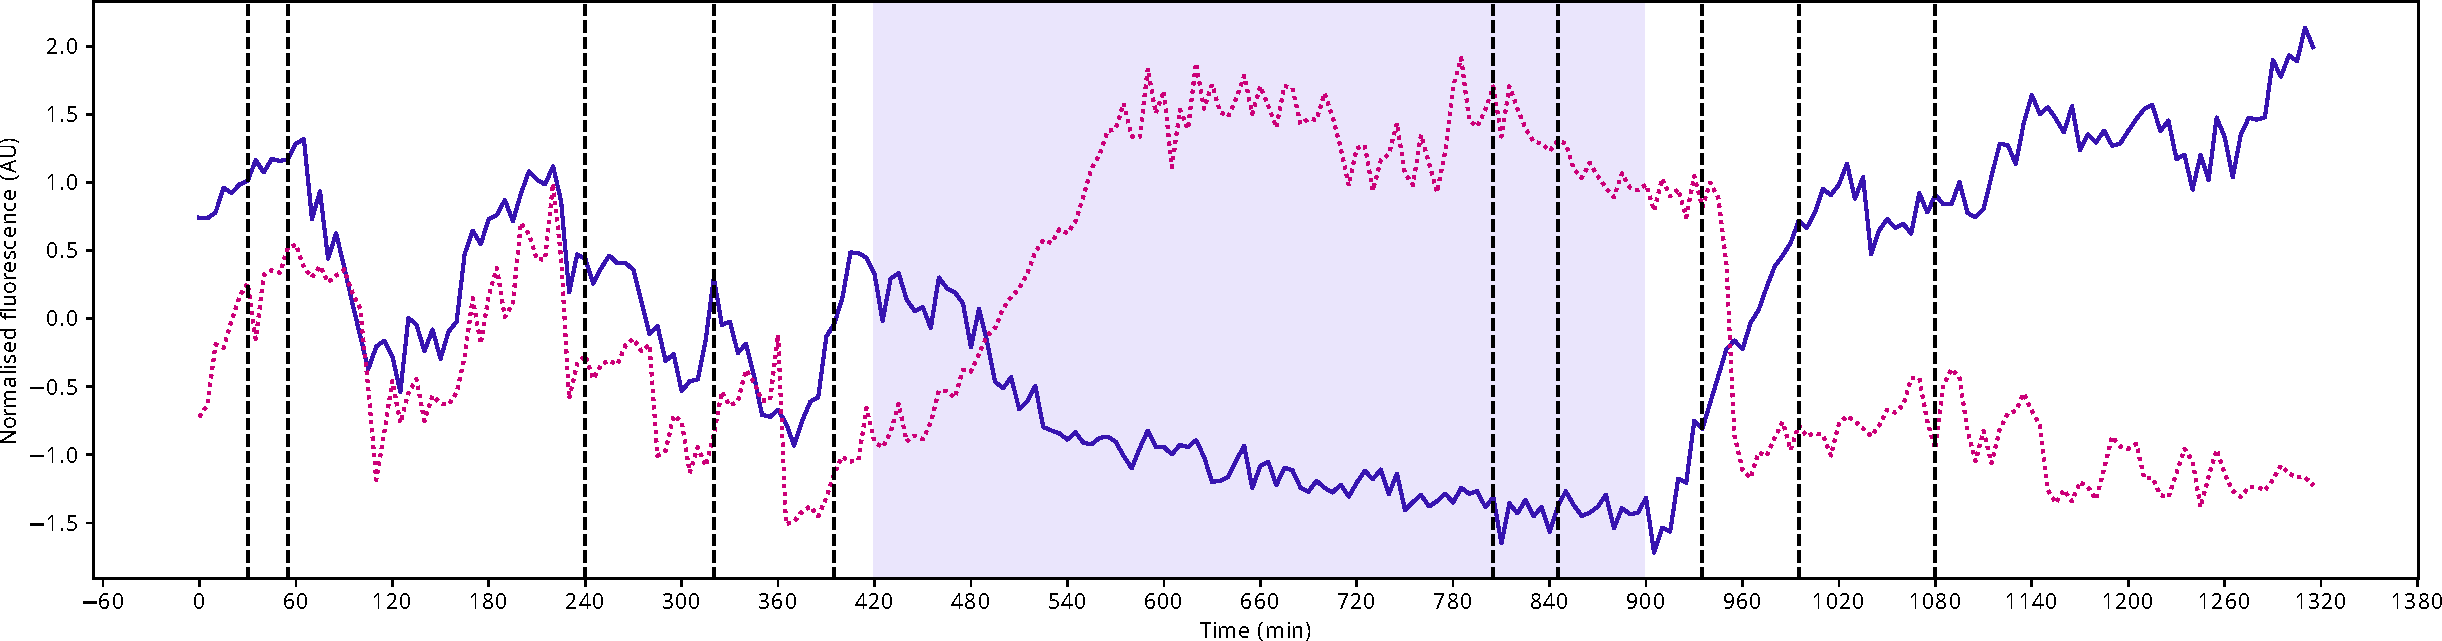
\includegraphics[width=\textwidth]{starvation_raw_13-07-02.pdf}
   \caption{
   }
   \label{fig:biology-starvation-raw-1}
  \end{subfigure}

  \begin{subfigure}[htpb]{1.0\textwidth}
   \centering
   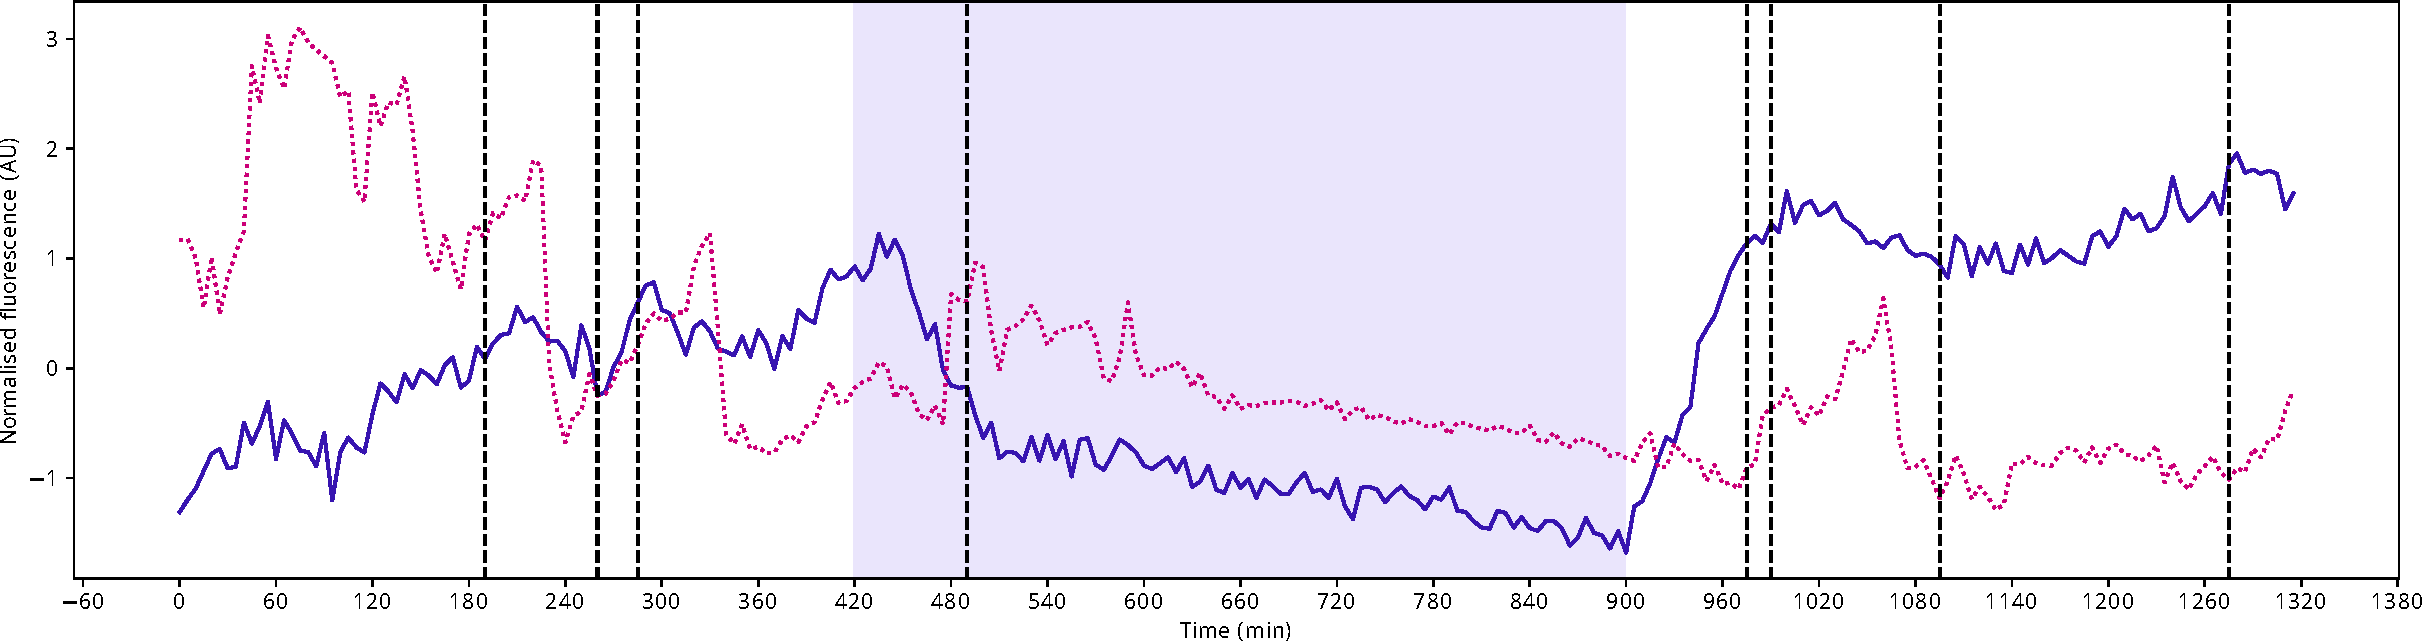
\includegraphics[width=\textwidth]{starvation_raw_13-39-01.pdf}
   \caption{
   }
   \label{fig:biology-starvation-raw-2}
  \end{subfigure}

  \caption{
    Upon starvation, histone 2B levels can remain at a high (~\ref{fig:biology-starvation-raw-1}) or low (~\ref{fig:biology-starvation-raw-2}) level.
    Note: unlike the other figures showing single-cell time series, the flavin and mCherry time series were normalised to give zero mean and standard deviation of 1 so that they can be plot on the same vertical axes, but the high-pass Butterworth filter was not applied to emphasise the trajectories of raw values.
  }
  \label{fig:biology-starvation-raw}
\end{figure}

On closer investigation of individual cell signals, I observe that histone 2B levels may remain at a high or low level upon starvation (figure~\ref{fig:biology-starvation-raw}).
These observations suggests that the cell remains in G1 or G2, or proceeds in the cell division cycle until it reaches G1 or G2, upon starvation.
% NEEDS MORE DISCUSSION, POSSIBLY A BIT MORE DATA ANALYSIS
This sheds light on how the relationship between the cell division cycle and the metabolic cycle may diverge during starvation, pointing to cellular mechanisms that may be responsible.


\begin{figure}
  \centering
  \begin{subfigure}[htpb]{0.9\textwidth}
   \centering
   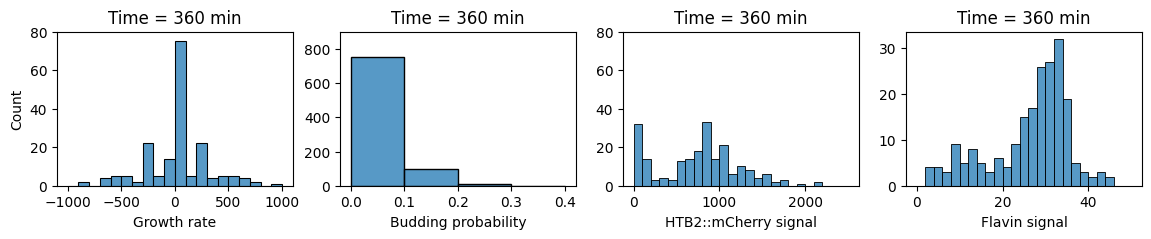
\includegraphics[width=\textwidth]{19972_distribs_0360}
   \caption{
     %foobar
     \SI{360}{\minute}
   }
   \label{fig:biology-starvation-distribs-0360}
  \end{subfigure}

  \begin{subfigure}[htpb]{0.9\textwidth}
   \centering
   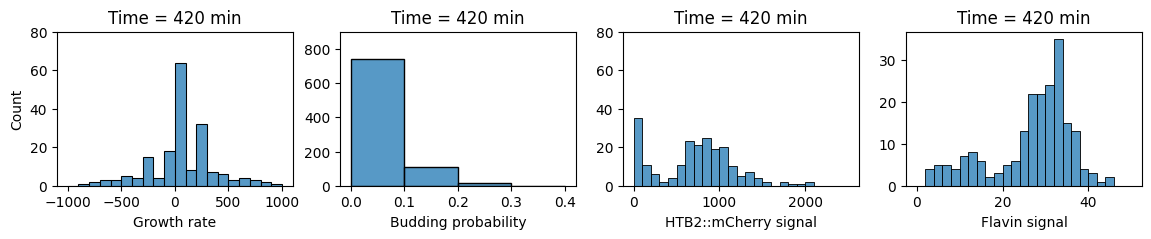
\includegraphics[width=\textwidth]{19972_distribs_0420}
   \caption{
     \SI{420}{\minute}
   }
   \label{fig:biology-starvation-distribs-0420}
  \end{subfigure}

  \begin{subfigure}[htpb]{0.9\textwidth}
   \centering
   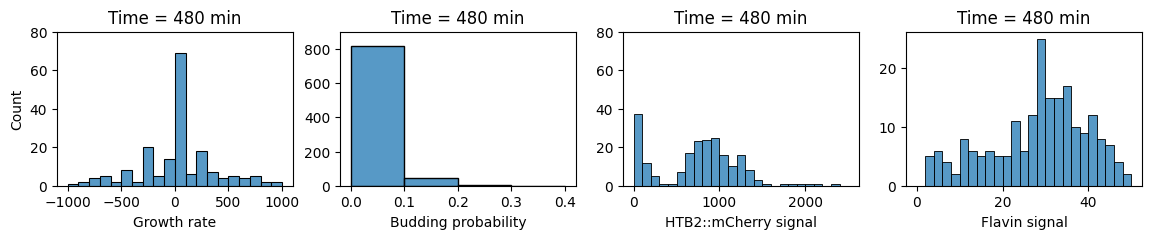
\includegraphics[width=\textwidth]{19972_distribs_0480}
   \caption{
     \SI{480}{\minute}
   }
   \label{fig:biology-starvation-distribs-0480}
  \end{subfigure}

  \begin{subfigure}[htpb]{0.9\textwidth}
   \centering
   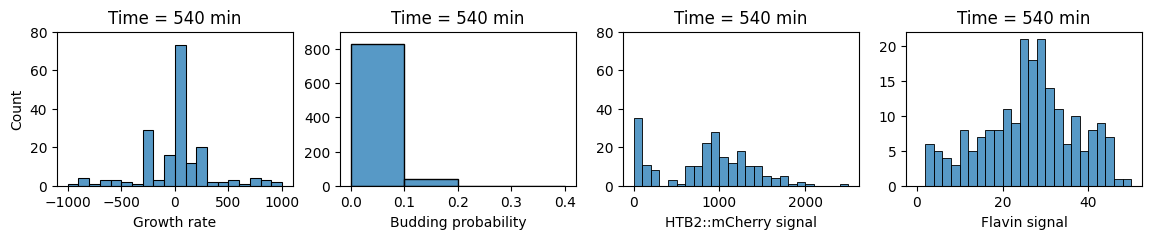
\includegraphics[width=\textwidth]{19972_distribs_0540}
   \caption{
     \SI{540}{\minute}
   }
   \label{fig:biology-starvation-distribs-0540}
  \end{subfigure}

  \begin{subfigure}[htpb]{0.9\textwidth}
   \centering
   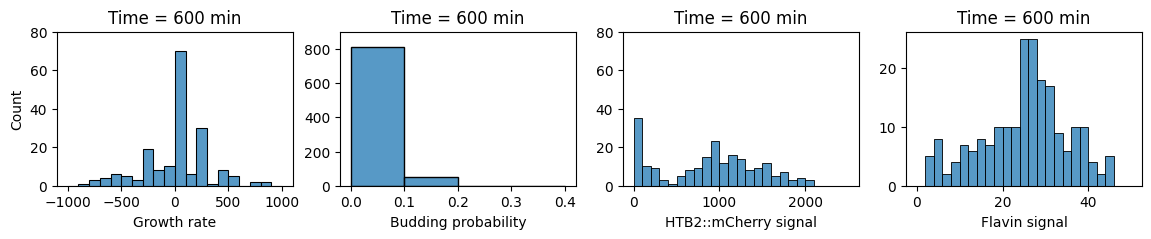
\includegraphics[width=\textwidth]{19972_distribs_0600}
   \caption{
     \SI{600}{\minute}
   }
   \label{fig:biology-starvation-distribs-0600}
  \end{subfigure}

  \begin{subfigure}[htpb]{0.9\textwidth}
   \centering
   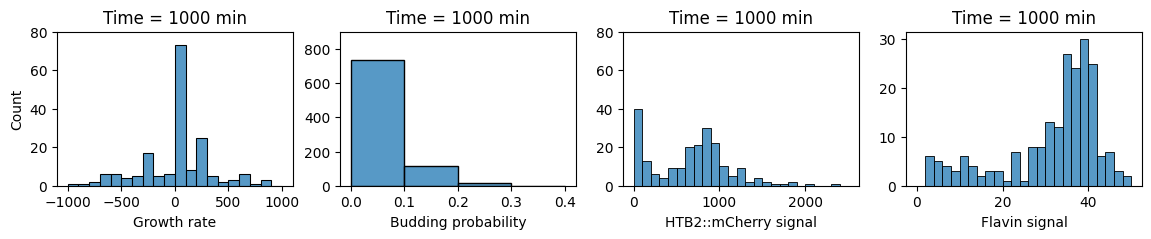
\includegraphics[width=\textwidth]{19972_distribs_1000}
   \caption{
     \SI{1000}{\minute}
   }
   \label{fig:biology-starvation-distribs-1000}
  \end{subfigure}

  \caption{
    Distribution of quantities at selected time points in the glucose-starvation experiment, starvation being \SIrange{420}{900}{\minute}.
    HTB2::mCherry and flavin signals were based on raw data extracted from the fluorescent images.
    Growth rate was calculated based on the rolling mean of the time point-to-time point change in cell volume estimated by \emph{aliby}, and the budding probability was calculated based on the rolling mean of the boolean vector that indicates the presence or absence of budding event over time.
  }
  \label{fig:biology-starvation-distribs}
\end{figure}


\begin{figure}
  \centering
  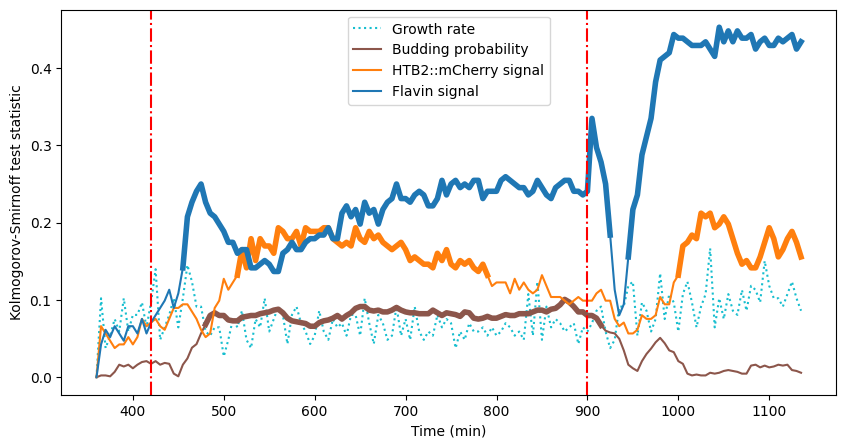
\includegraphics[width=\textwidth]{19972_ks_highlight}
  \caption{
    Glucose-starvation experiment.
    For each quantity, the Kolmogorov-Smirnov test statistics from two-tailed tests between the distribution at \SI{360}{\minute} and the distribution at each time point of interest is shown.
    The null hypothesis for each test is that the two samples are drawn from the same probability distribution, and thick lines indicate where the hypothesis is rejected ($p < 0.05$).
    Vertical lines (red) indicate changes in nutrient conditions.
  }
  \label{fig:biology-starvation-ks}
\end{figure}

% This sentence is difficult to understand.  Deal with it during the editing phase.
To extend information about the cell division cycle phase each cell is upon and during starvation across the population, I show the distribution of the raw HTB2::mCherry signals at time points of interest in the experiment (figure~\ref{fig:biology-starvation-distribs}).
The distributions of growth rates, budding probability, and raw flavin intensity are also shown.
To quantify how the distributions of these quantities change over time, I performed a two-tailed Kolmogorov-Smirnov test between a pre-starvation reference time each time point of interest over the course of the experiment (figure~\ref{fig:biology-starvation-ks}).

Consistent with figure~\ref{fig:biology-starvation-budprob}, the distribution of budding probability skews more towards zero during starvation, indicating sparse budding, and then budding resumes after starvation.
During starvation, initially the distribution of HTB2::mCherry signals remain the same, but after approximately \SI{2}{\hour}, it becomes more spread out.
This pattern suggests a delay in the effect of starvation on the progress of the cell division cycle as cell division cycles progress to their next available checkpoints.
Interestingly, the distribution of flavin signals skews to lower values during starvation, before recovering after starvation, and this suggests a more reduced cellular oxidation state during starvation.
% ...Needs more interpretation.  What does this suggest about the cell biology during starvation?  Is there a link to the literature?


\section{Effect of carbon source on YMC.}
\label{sec:biology-carbon}

To extend on the idea that the metabolic cycle responds to nutrient conditions and accordingly adjusts the cell's metabolism and cell division cycle, I performed experiments in which I culture cells in pyruvate and in a growth-limiting glucose concentration.
These experiments are important as they confirm conclusions about varying nutrient conditions made by \textcite{papagiannakisAutonomousMetabolicOscillations2017}, but using flavin autofluorescence and in more carbon sources.

\begin{figure}
  \centering
  \begin{subfigure}[htpb]{1.0\textwidth}
   \centering
   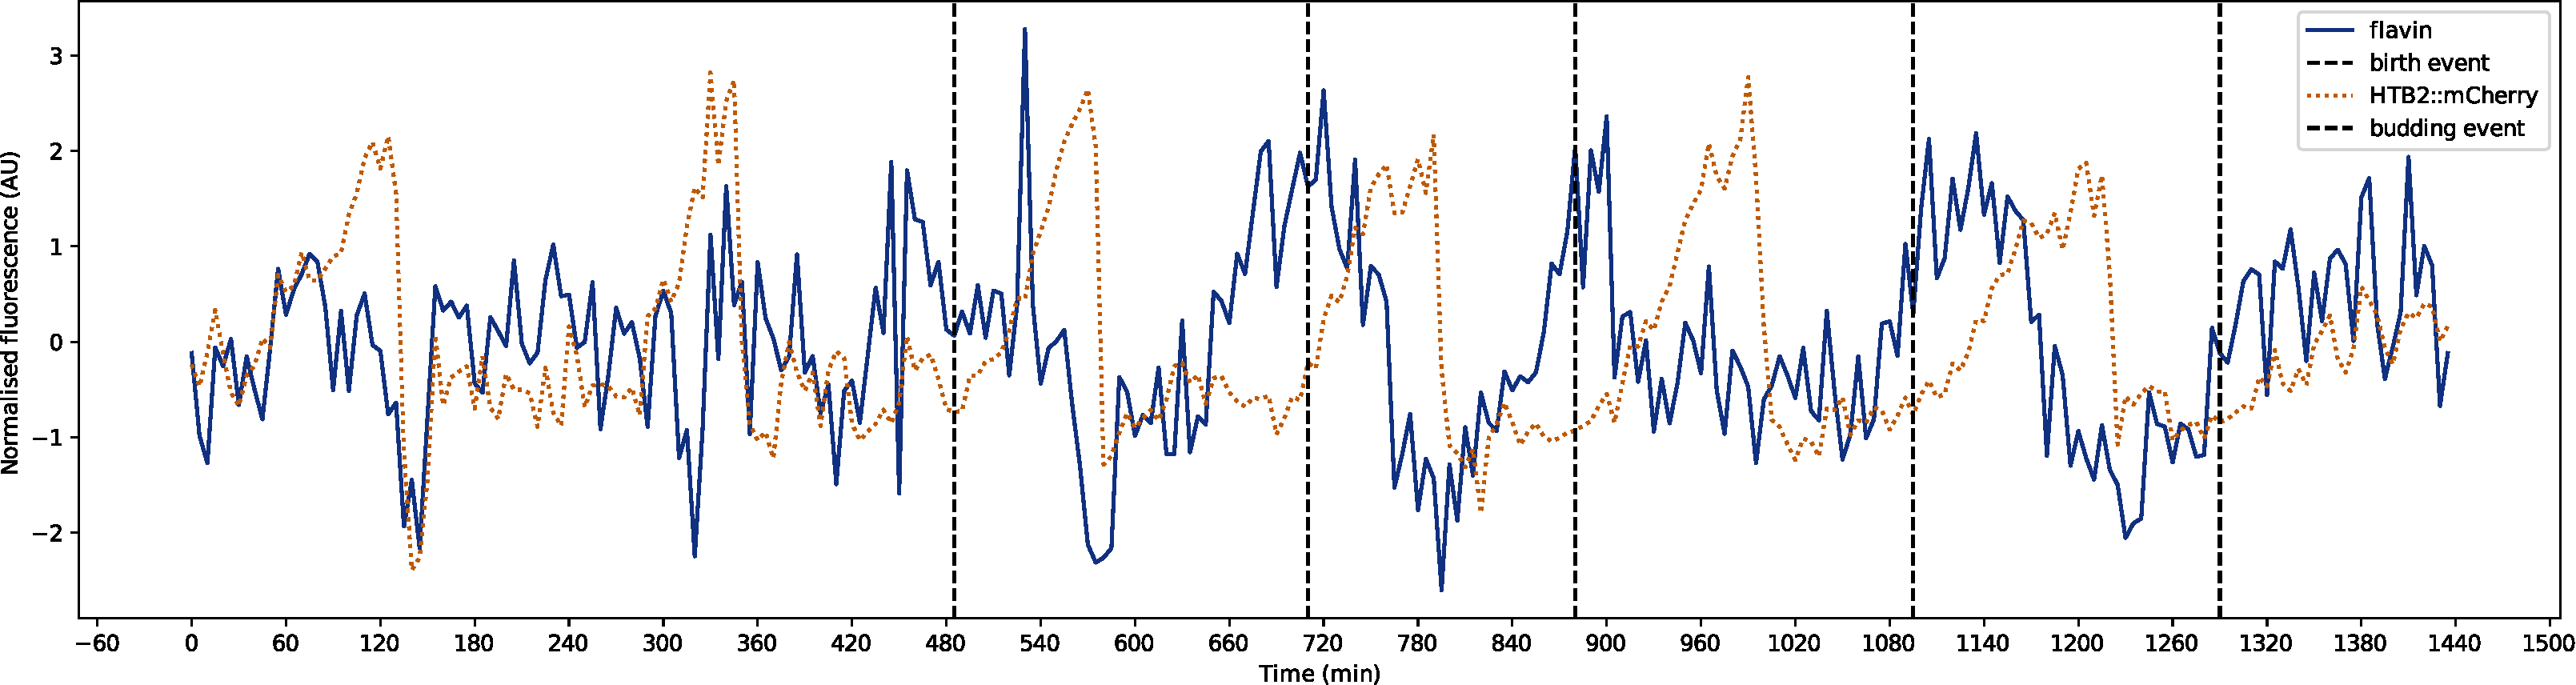
\includegraphics[width=\textwidth]{pyruvate_single_birth_plot_edit.pdf}
   \caption{
     Oscillations of flavin fluorescence lengthen when cells are cultivated in \SI{20}{\gram~\litre^{-1}} pyruvate while the duration of S/M phase stays constant.
     %Figure shows sample flavin fluorescence levels (purple) and histone 2B localisation (pink) in single cells.
     %Vertical lines (black) indicate budding.
   }
   \label{fig:biology-pyruvate-single}

  \end{subfigure}
  \begin{subfigure}[t]{0.45\textwidth}
   \centering
   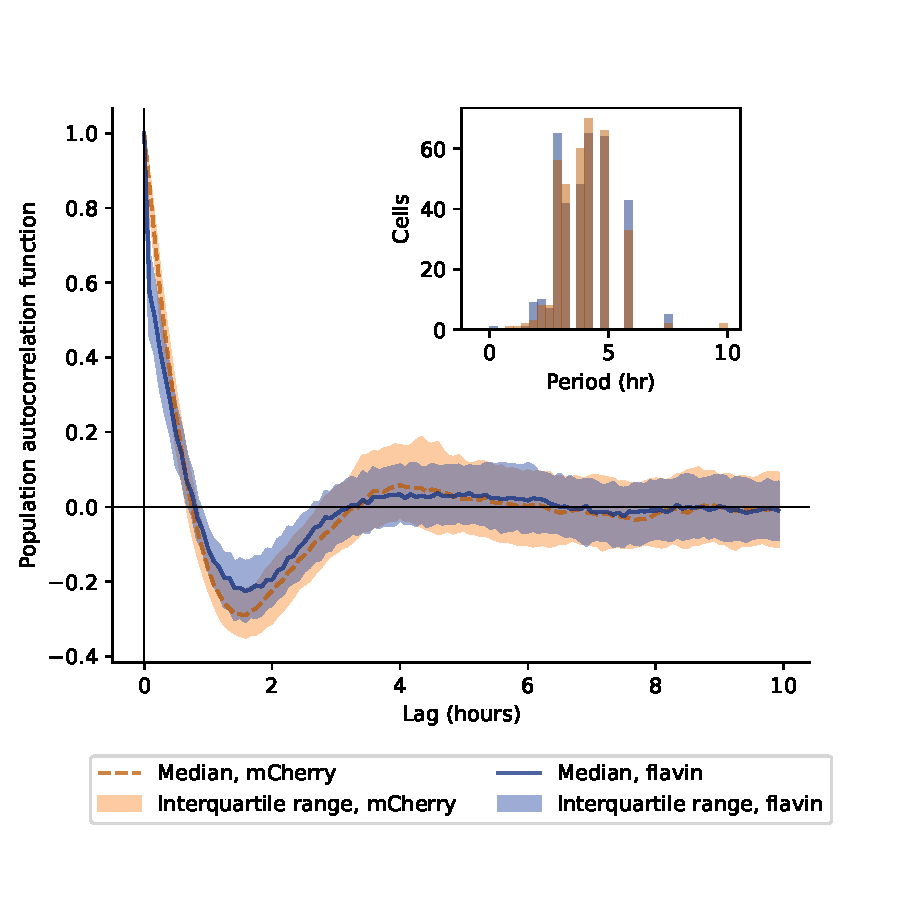
\includegraphics[width=\textwidth]{htb2mCherry_31594_12.pdf}
   \caption{
     Autocorrelation functions and periods determined by Fourier spectrum of flavin fluorescence and histone 2B levels.
     This figure indicates that the cells' metabolic cycles and cell division cycles are both consistently approximately 4 hours long.
   }
   \label{fig:biology-pyruvate-acf}
  \end{subfigure}%
  \begin{subfigure}[t]{0.45\textwidth}
   \centering
   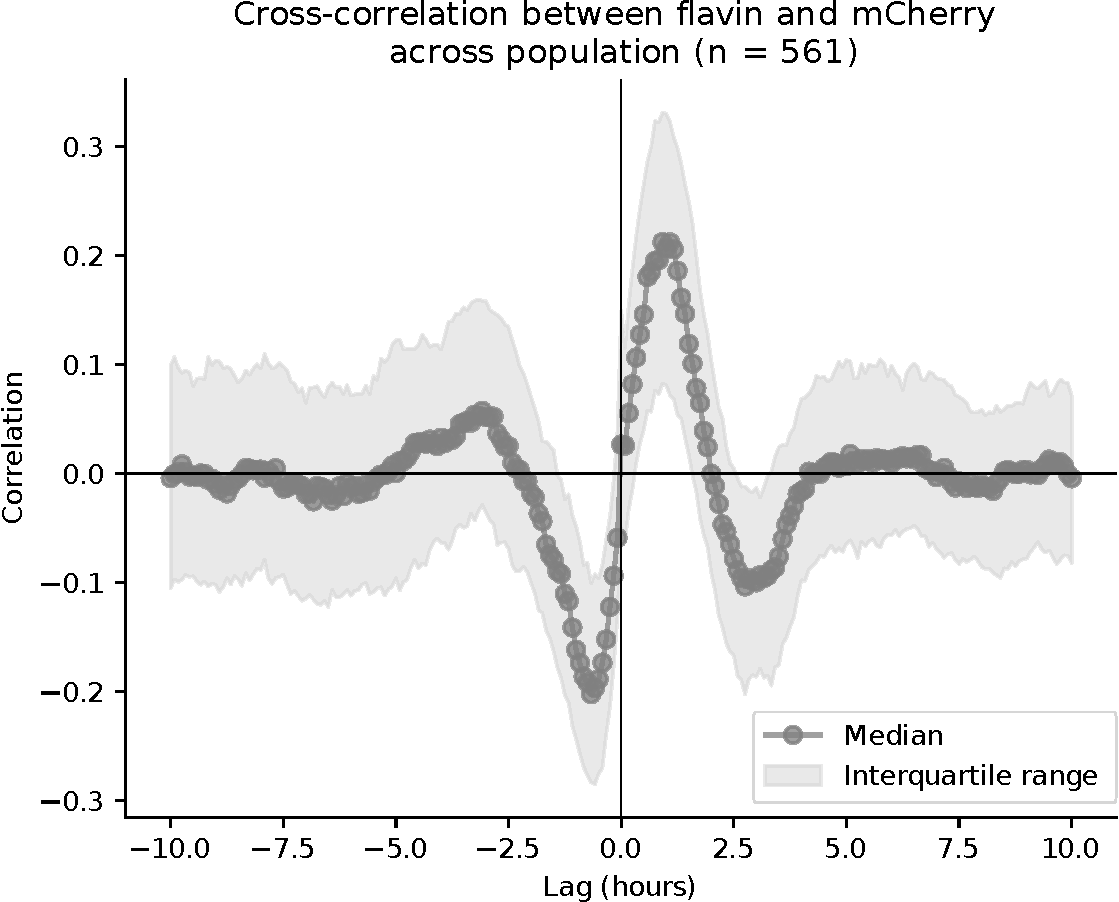
\includegraphics[width=\textwidth]{pyruvate_xcf_edit.pdf}
   \caption{
    Cross-correlation between flavin and histone 2B signals, indicating that histone levels peak 1 hour after flavin fluorescence peaks.
   }
   \label{fig:biology-pyruvate-xcf}
  \end{subfigure}

  \caption{
    When cultivated in \SI{20}{\gram~\litre^{-1}} pyruvate, cells show longer metabolic cycles while the S/M phase of the cell division cycle remains the same length and the G1 phase lengthens.
  }
  \label{fig:biology-pyruvate}
\end{figure}

FY4 HTB2::mCherry cells were grown in minimal media supplemented with \SI{20}{\gram~\litre^{-1}} sodium pyruvate to provide a non-fermentable carbon source.
In this condition, the cells showed longer metabolic cycles and cell division cycles, of approximately \SI{4}{\hour} (figure~\ref{fig:biology-pyruvate}).
In addition, there were more cases in which the flavin signal peaks without a budding event (supplementary figure ...).
Furthermore, the synchrony between the two oscillators remain, but with a longer lag of the cell division cycle with respect to the metabolic cycle (figure~\ref{fig:biology-pyruvate-xcf}).
However, the flavin cycles seem to be less robust: cycles are not so regular over long periods of time, as evidenced by a lack of repeated oscillations in the cross-correlation function.
Figure~\ref{fig:biology-pyruvate-single} shows that the longer cell division cycles were because of longer G1 phases but unchanged S/M phases, as evidenced by the longer flat regions of the HTB2::mCherry signal.
This observation is consistent with the knowledge on the cell division cycle, %[CITATION NEEDED]
and it draws comparison with the discussion about the change in lengths of phases in the metabolic cycle. %[ELABORATE MORE -- CONSULT INTRO.  I'm thinking of the Mellor/Slavov & Botstein stuff]
% THIS THEN WARRANTS DISCUSSION.

% COULD DO:
% (Add statistical tests to reject the null hypothesis that the mean duration of metabolic cycles in pyruvate is equal to the mean duration of metabolic cycles in high glucose.)


\begin{figure}
  \centering
  \begin{subfigure}[htpb]{1.0\textwidth}
   \centering
   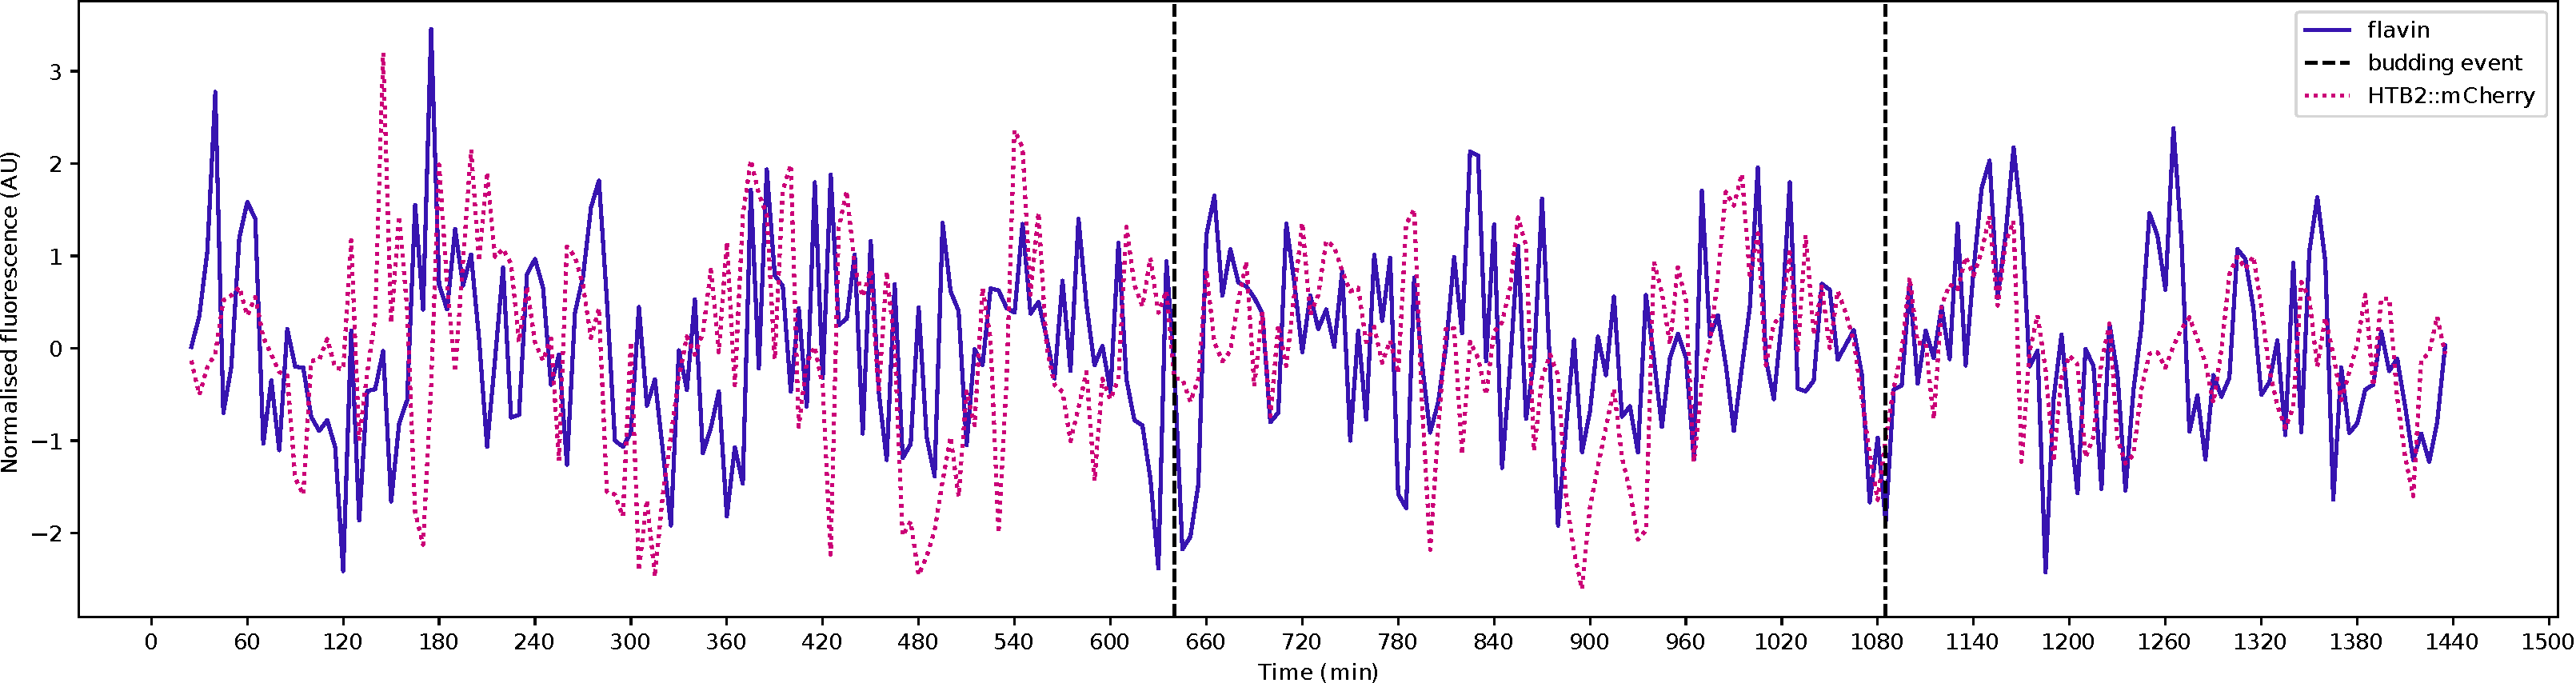
\includegraphics[width=\textwidth]{limiting_single_birth_plot_edit.pdf}
   \caption{
     Oscillations of flavin fluorescence are noisier when cells are cultivated in \SI{10}{\milli\gram~\litre^{-1}} glucose while cells show minimal growth or division.
     %Figure shows sample flavin fluorescence (purple) and histone 2B (pink) level in a single cell grown in \SI{10}{\milli\gram~\litre^{-1}}.
     %Vertical dashed lines (black) indicate budding.
   }
   \label{fig:biology-lowglc-single}
  \end{subfigure}

  \begin{subfigure}[htpb]{0.7\textwidth}
   \centering
   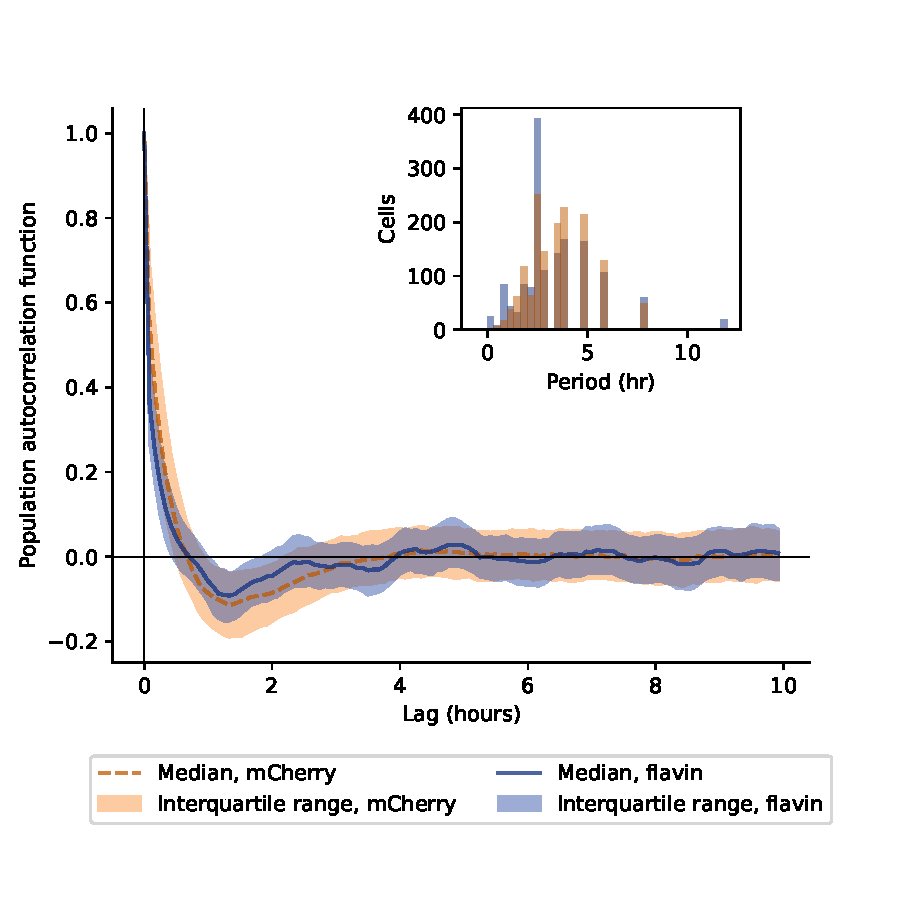
\includegraphics[width=\textwidth]{htb2mCherry_31492_12.pdf}
   \caption{
     Autocorrelation functions and periods determined by Fourier spectrum of flavin fluorescence and histone 2B levels.
     This figure indicates that the cells' metabolic cycles are approximately \SI{2.5}{\hour} long, but the duration of the cell division cycle is not robust nor consistent across the population.
   }
   \label{fig:biology-lowglc-acf}
  \end{subfigure}

  \begin{subfigure}[t]{0.3\textwidth}
   \centering
   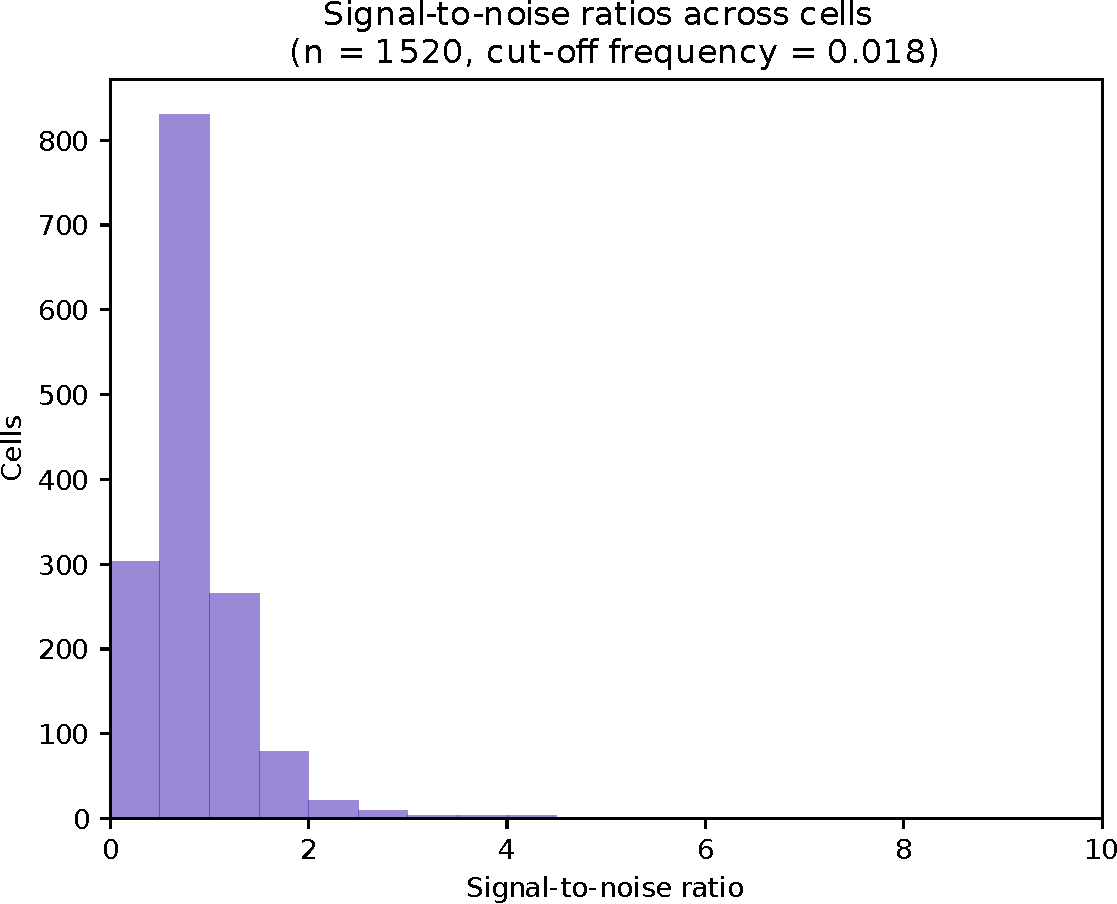
\includegraphics[width=\textwidth]{limiting_snr_edit.pdf}
   \caption{
     Signal-to-noise ratios, \SI{10}{\milli\gram~\litre^{-1}} glucose.
     %Distribution of signal-to-noise ratios computed for each flavin time series derived from cells cultivated in \SI{10}{\milli\gram~\litre^{-1}}, showing that most cells have noisy signals and thus implying low-amplitude metabolic cycles.
   }
   \label{fig:biology-lowglc-snr}
  \end{subfigure}%
  \begin{subfigure}[t]{0.3\textwidth}
   \centering
   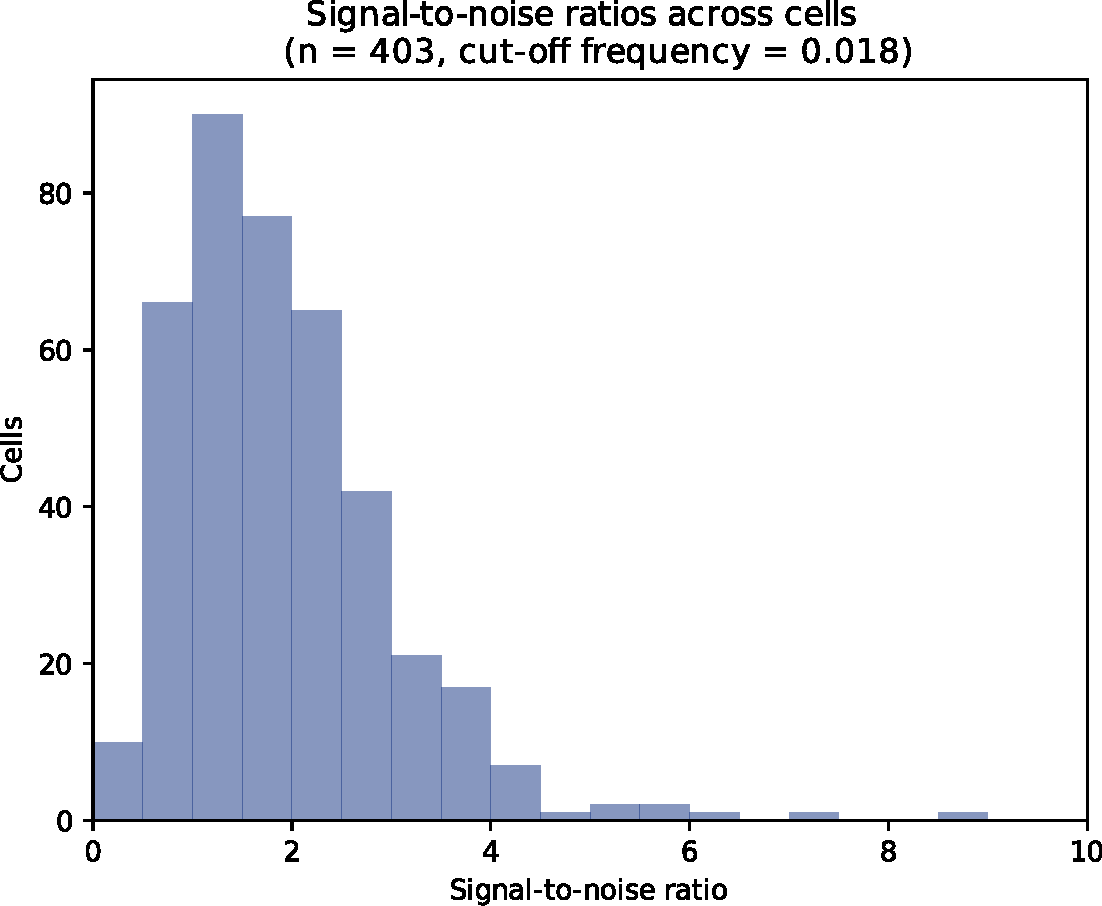
\includegraphics[width=\textwidth]{pyruvate_snr_edit.pdf}
   \caption{
     Signal-to-noise ratios, \SI{20}{\gram~\litre^{-1}} pyruvate.
    %Distribution of signal-to-noise ratios computed for each flavin time series derived from cells cultivated in \SI{20}{\gram~\litre^{-1}} pyruvate, showing that cells have higher-quality signals.
   }
   \label{fig:biology-pyruvate-snr}
  \end{subfigure}%
  \begin{subfigure}[t]{0.3\textwidth}
   \centering
   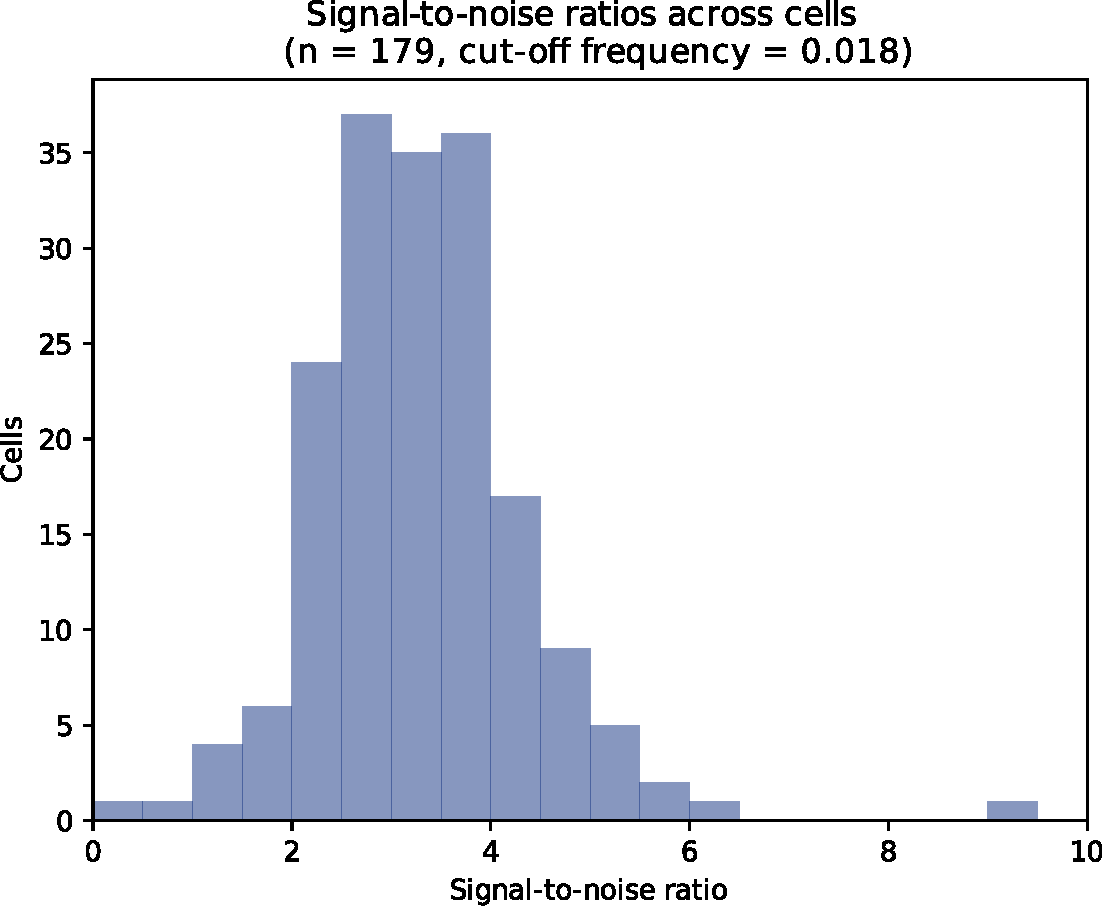
\includegraphics[width=\textwidth]{glucose_snr_edit.pdf}
   \caption{
     Signal-to-noise ratios, \SI{20}{\gram~\litre^{-1}} glucose.
    %Distribution of signal-to-noise ratios computed for each flavin time series derived from cells cultivated in \SI{20}{\gram~\litre^{-1}} glucose, showing that cells have higher-quality signals.
   }
   \label{fig:biology-highglc-snr}
  \end{subfigure}

  \caption{
    When cultivated in growth-limiting (\SI{10}{\milli\gram~\litre^{-1}}) glucose, cells show lower-quality metabolic cycles with lower amplitudes, as suggested by the distributions of signal-to-noise ratios computed for each flavin time series (\ref{fig:biology-lowglc-snr},~\ref{fig:biology-pyruvate-snr},~\ref{fig:biology-highglc-snr}).
  }
  \label{fig:biology-lowglc}
\end{figure}


% TODO: Plot on same axes, to strengthen comparison between conditions?
\begin{figure}
  \centering
  \begin{subfigure}[htpb]{0.45\textwidth}
   \centering
   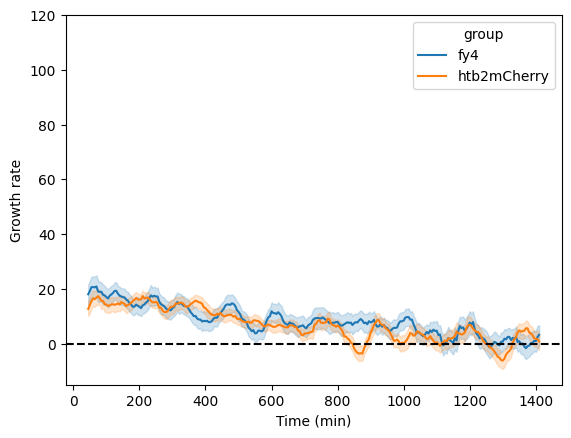
\includegraphics[width=\textwidth]{allstrains_31492_gr}
   \caption{
     Growth rate, low glucose
   }
   \label{fig:biology-lowglc-gr}
  \end{subfigure}%
  \begin{subfigure}[htpb]{0.45\textwidth}
   \centering
   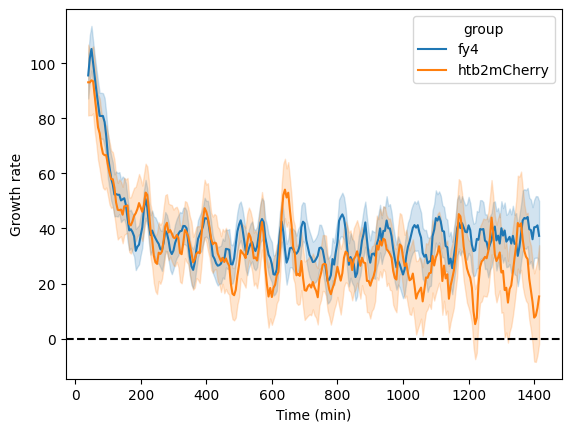
\includegraphics[width=\textwidth]{allstrains_26643_gr}
   \caption{
     Growth rate, high glucose
   }
   \label{fig:biology-highglc-gr}
  \end{subfigure}

  \begin{subfigure}[htpb]{0.45\textwidth}
   \centering
   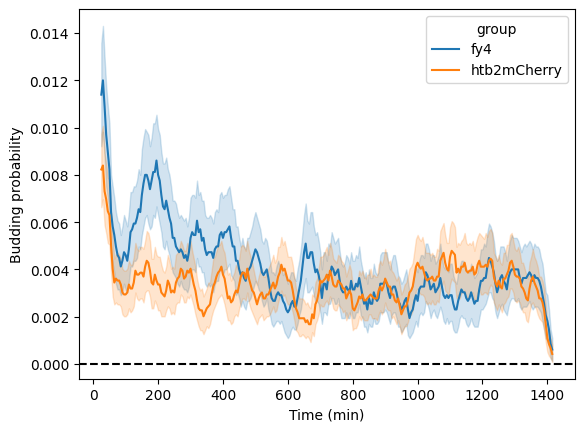
\includegraphics[width=\textwidth]{allstrains_31492_budprob}
   \caption{
     Budding probability, low glucose
   }
   \label{fig:biology-lowglc-budprob}
  \end{subfigure}%
  \begin{subfigure}[htpb]{0.45\textwidth}
   \centering
   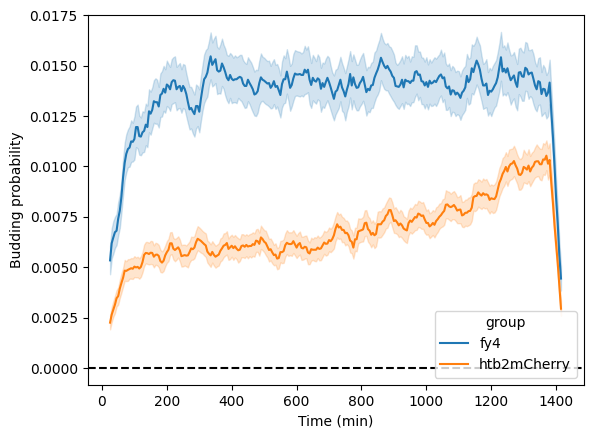
\includegraphics[width=\textwidth]{allstrains_26643_budprob}
   \caption{
     Budding probability, high glucose
   }
   \label{fig:biology-highglc-gr}
  \end{subfigure}

  \caption{
    Growth rates and budding probabilities of cells in limiting glucose (\SI{10}{\milli\gram~\litre^{-1}}) compared to high glucose \SI{20}{\gram~\litre^{-1}}.
    Mean growth rate and budding probability of FY4 (blue) and HTB2::mCherry (orange) strains over time, with 95\% confidence intervals shown (shaded).
  }
  \label{fig:biology-lowglc-gr-budprob}
\end{figure}
% COULD DO:
%(Add statistical tests to reject the null hypothesis that the distribution of SNRs are the same between the three nutrient conditions.)

Next, I performed an experiment with limiting glucose to emulate low-glucose conditions one may encounter in a chemostat.
When FY4 HTB2::mCherry cells were grown in minimal media supplemented with \SI{10}{\milli\gram~\litre^{-1}} glucose, the cells showed longer metabolic cycles and an relative absence of cell division (figure~\ref{fig:biology-lowglc-single}).
Figure~\ref{fig:biology-lowglc-gr-budprob} confirms that the growth rate and the budding probability of cells on limiting glucose is lower than on high glucose (\SI{20}{\gram~\litre^{-1}}).
Furthermore, the flavin signals are of low amplitude and low quality, as evidenced by the low signal-to-noise ratios (figure~\ref{fig:biology-lowglc-snr}).
Though less robust, the metabolic cycles follow an approximately \SI{2.5}{\hour} long period, but the duration of the cell division cycle is not robust nor consistent across the population (figure~\ref{fig:biology-lowglc-acf}); this gives an additional situation where the synchrony between the metabolic cycle and the cell division cycle is lost.

% In contrast to 20 g/L glucose in which metabolic cycles were asynchronous, in these conditions there is some degree of metabolic cycle synchrony between cells. \textbf{(add figures)}

% TODO: How are these linked to Papagiannakis et al.?  Am I getting the same conclusions?  Also -- space to discuss the 10-hour oscillations in chemostats in slow dilution rates.


%\section[Potassium-deficient media]{Do single-cell flavin traces recapitulate dissolved-oxygen YMCs in chemostats? -- potassium-deficient media}
\section{Metabolic cycles persist in potassium-deficient media}
\label{sec:biology-potassium_deficient}

To address whether single-cell flavin traces from my microfluidics experiments recapitulate dissolved-oxygen yeast metabolic cycles in chemostats, I turn to several chemostat-based studies that demonstrate nutrient or genetic perturbations that severely affect the metabolic cycle.
This is important in showing that the single-cell metabolic cycle and the chemostat metabolic cycle are the same cycle, or to prove otherwise.
Chemostat experiments obscure the behaviour of individual cells.
My single-cell microfluidics experiments should produce a more detailed picture of how changes to the metabolic cycle affect the coarse-grained readouts in chemostat-based studies.

\begin{figure}
  \centering
  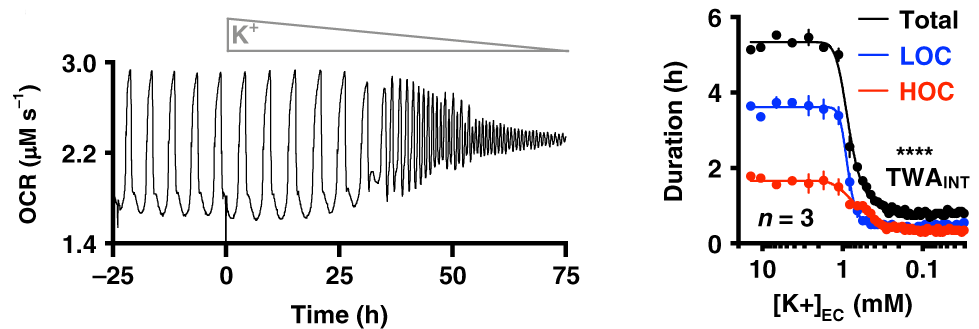
\includegraphics[width=0.7\textwidth]{oneillEukaryoticCellBiology2020_4_adapted.png}
  \caption{
    Decreasing extracellular potassium (\ce{K+}) concentration shortens, then under \SI{1}{\milli\molar}, destroys metabolic oscillations in the chemostat.
    Adapted from \textcite{oneillEukaryoticCellBiology2020}.
  }
  \label{fig:biology-kdeficient-oneill}
\end{figure}

First, I consider potassium-deficient media.
\textcite{oneillEukaryoticCellBiology2020} suggest that as potassium is gradually replaced with sodium in chemostat culture media, the amplitude of dissolved-oxygen oscillations decrease until they disappear altogether (figure~\ref{fig:biology-kdeficient-oneill}).


\begin{figure}
  \centering
  \begin{subfigure}[htpb]{1.0\textwidth}
   \centering
   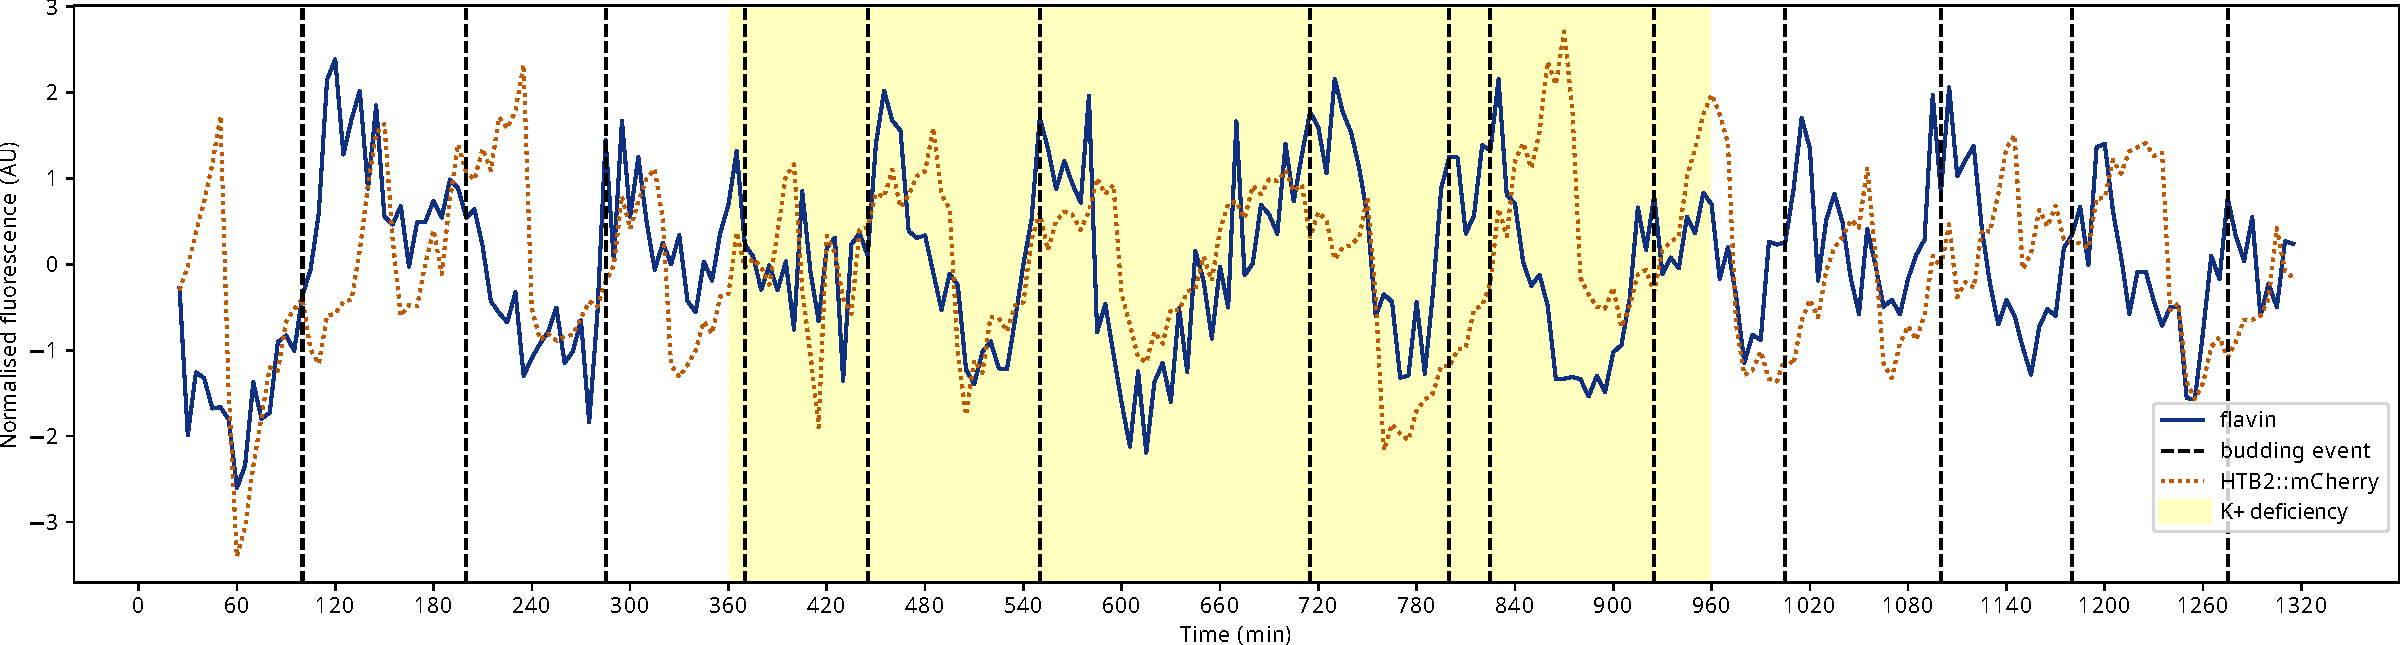
\includegraphics[width=\textwidth]{htb2mCherry_613_plots_single_htb2mCherry012_90_2_adapted.pdf}
   \caption{
     Flavin fluorescence and cell division cycles are maintained before, during, and after perfusion of potassium-deficient nutrient media (FY4 HTB2::mCherry).
   }
   \label{fig:biology-kdeficient-single}
  \end{subfigure}

  \begin{subfigure}[htpb]{0.7\textwidth}
   \centering
   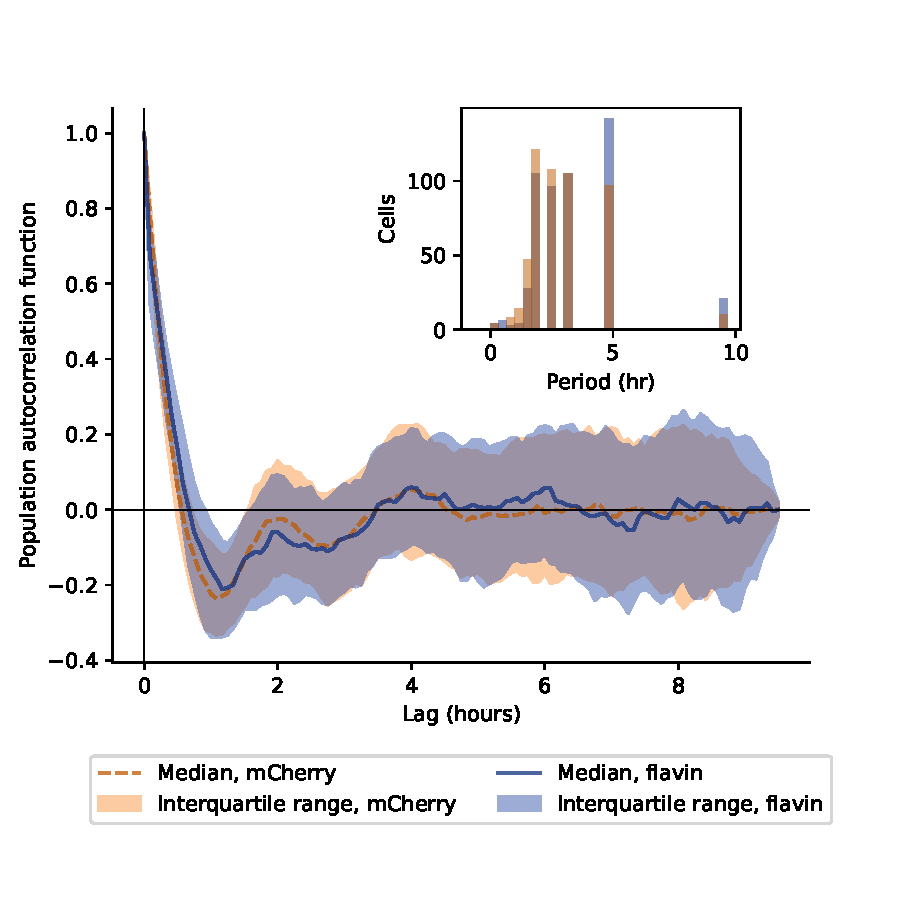
\includegraphics[width=\textwidth]{htb2mCherry_613_12.pdf}
   \caption{
     Autocorrelation functions and periods determined by Fourier spectrum of flavin fluorescence and histone 2B levels.
     Only time points during potassium-deficiency were used in the calculations.
     This figure indicates that the cells' metabolic cycles and cell division cycles are both consistently 120 minutes long.
   }
   \label{fig:biology-kdeficient-acf}
  \end{subfigure}

  \caption{
    When grown in potassium-deficient media and with \SI{20}{\gram~\litre^{-1}} glucose as a carbon source, cells showed metabolic cycles, contrary to \textcite{oneillEukaryoticCellBiology2020}
  }
  \label{fig:biology-kdeficient}
\end{figure}

I cultured FY4 HTB2::mCherry cells with minimal media supplemented with \SI{20}{\gram~\litre^{-1}} glucose.
The minimal media contains \ce{KH2PO4} as a potassium salt, so I prepared an alternative media formulation with the salt replaced with \ce{NaH2PO4} at the same molarity.
During the microfluidics experiment, cells were grown on normal growth medium for \SI{6}{\hour} before being abruptly switched to potassium-free medium for \SI{10}{\hour} and then resumed to normal growth medium for \SI{6}{\hour}.
In contrast to what \textcite{oneillEukaryoticCellBiology2020} would suggest, I observe that flavin metabolic oscillations are generated in potassium-deficient media, with synchronised cell division cycles (figure~\ref{fig:biology-kdeficient-single}).
Such cycles are longer and generated less reliably as in the normal growth medium (figure~\ref{fig:biology-kdeficient-acf}).


\begin{figure}
  \centering
  \begin{subfigure}[htpb]{0.7\textwidth}
   \centering
   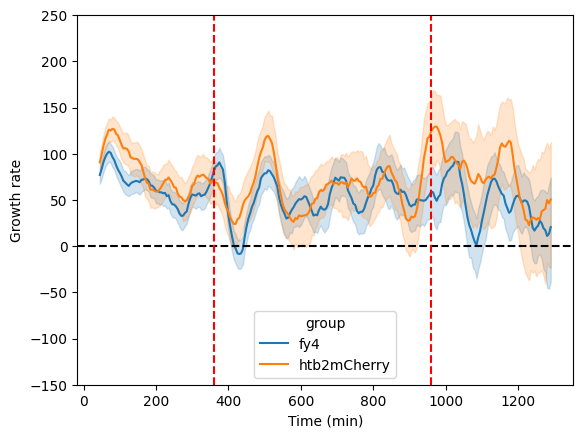
\includegraphics[width=\textwidth]{allstrains_613_gr}
   \caption{
     Growth rate
   }
   \label{fig:biology-kdeficient-gr}
  \end{subfigure}

  \begin{subfigure}[htpb]{0.7\textwidth}
   \centering
   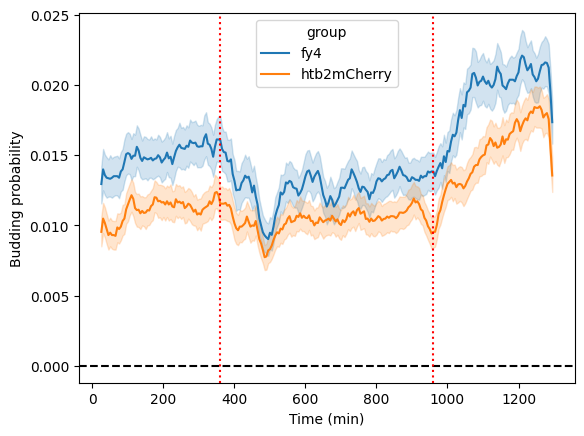
\includegraphics[width=\textwidth]{allstrains_613_budprob}
   \caption{
     Budding probability
   }
   \label{fig:biology-kdeficient-budprob}
  \end{subfigure}

  \caption{
    Mean growth rate and budding probability of FY4 (blue) and HTB2::mCherry (orange) strains over time during the potassium-deficiency experiment, with 95\% confidence intervals shown (shaded).
    Vertical lines (red) show changes in nutrient media.
  }
  \label{fig:biology-kdeficient-gr-budprob}
\end{figure}

In addition, although there was a sharp drop in growth rate in response to the abrupt change to the potassium-deficient medium (figure~\ref{fig:biology-kdeficient-gr}), the growth rate recovered soon after.
The budding probability only showed a slight drop during potassium-deficiency (figure~\ref{fig:biology-kdeficient-budprob}), in contrast to a near-zero drop under glucose starvation (figure~\ref{fig:biology-starvation-budprob}).


\begin{figure}
  \centering
  \begin{subfigure}[htpb]{0.9\textwidth}
   \centering
   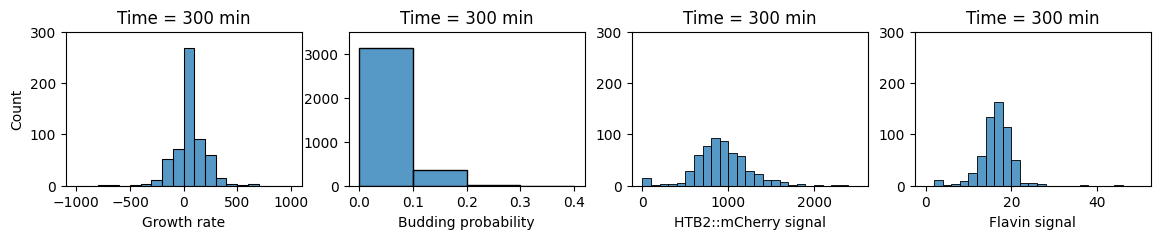
\includegraphics[width=\textwidth]{613_distribs_0300}
   \caption{
     \SI{300}{\minute}
   }
   \label{fig:biology-kdeficient-distribs-0300}
  \end{subfigure}

  \begin{subfigure}[htpb]{0.9\textwidth}
   \centering
   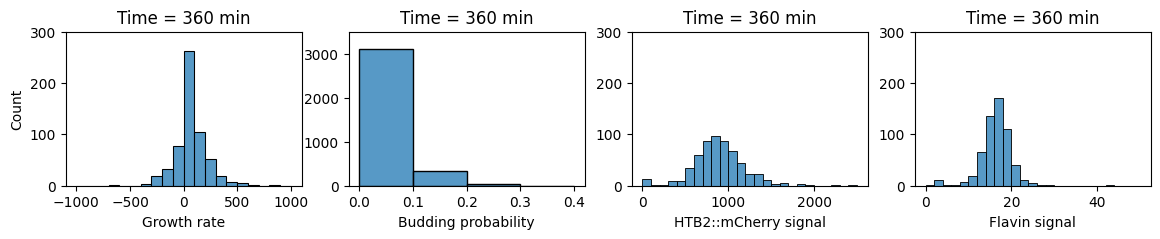
\includegraphics[width=\textwidth]{613_distribs_0360}
   \caption{
     \SI{360}{\minute}
   }
   \label{fig:biology-kdeficient-distribs-0360}
  \end{subfigure}

  \begin{subfigure}[htpb]{0.9\textwidth}
   \centering
   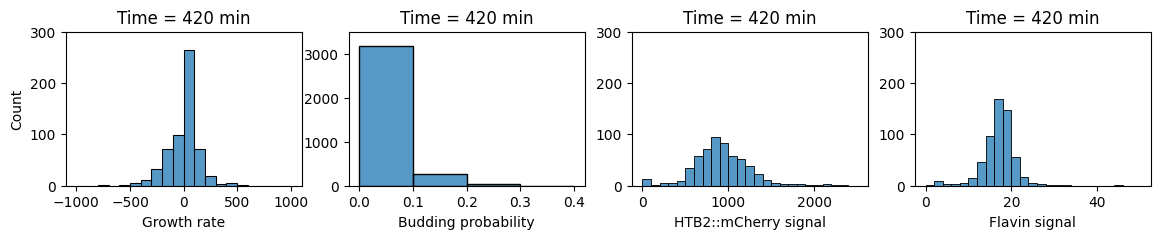
\includegraphics[width=\textwidth]{613_distribs_0420}
   \caption{
     \SI{420}{\minute}
   }
   \label{fig:biology-kdeficient-distribs-0420}
  \end{subfigure}

  \begin{subfigure}[htpb]{0.9\textwidth}
   \centering
   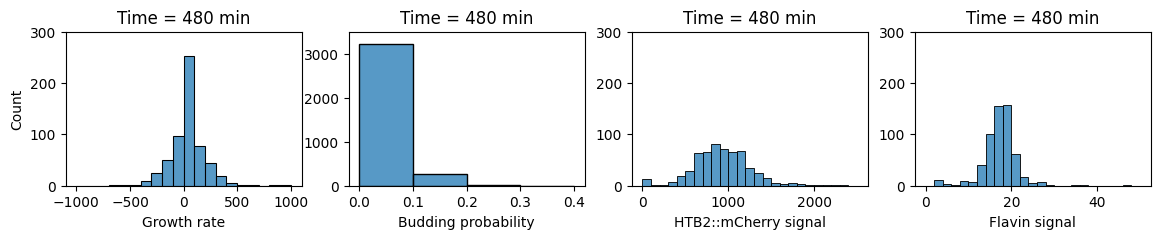
\includegraphics[width=\textwidth]{613_distribs_0480}
   \caption{
     \SI{480}{\minute}
   }
   \label{fig:biology-kdeficient-distribs-0480}
  \end{subfigure}

  \begin{subfigure}[htpb]{0.9\textwidth}
   \centering
   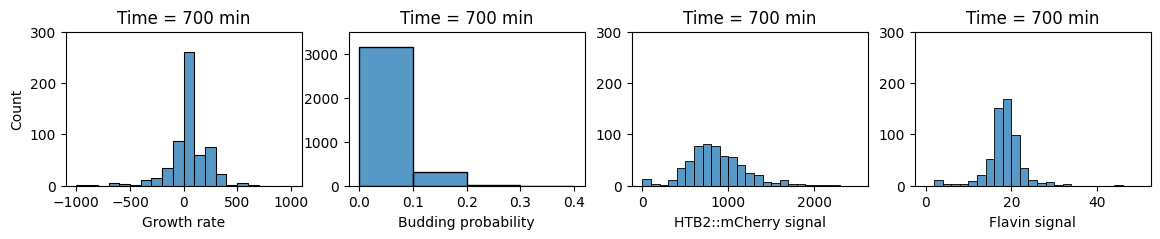
\includegraphics[width=\textwidth]{613_distribs_0700}
   \caption{
     \SI{700}{\minute}
   }
   \label{fig:biology-kdeficient-distribs-0700}
  \end{subfigure}

  \begin{subfigure}[htpb]{0.9\textwidth}
   \centering
   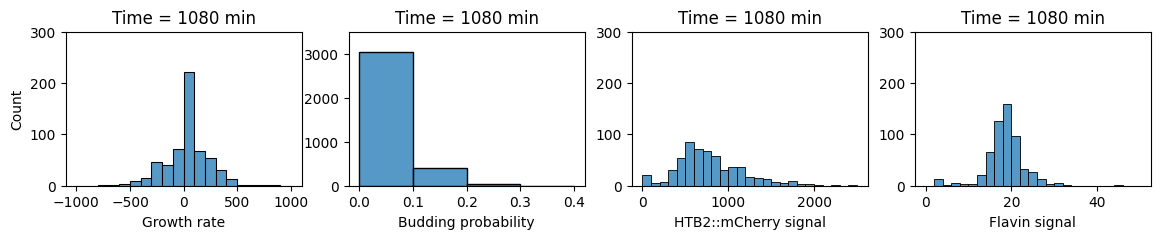
\includegraphics[width=\textwidth]{613_distribs_1080}
   \caption{
     \SI{1080}{\minute}
   }
   \label{fig:biology-kdeficient-distribs-1080}
  \end{subfigure}

  \caption{
    Distribution of quantities at selected time points in the potassium-deficiency experiment, potassium-deficiency being \SIrange{360}{960}{\minute}.
    HTB2::mCherry and flavin signals were based on raw data extracted from the fluorescent images.
    Growth rate was calculated based on the rolling mean of the time point-to-time point change in cell volume estimated by \emph{aliby}, and the budding probability was calculated based on the rolling mean of the boolean vector that indicates the presence or absence of budding event over time.
  }
  \label{fig:biology-kdeficient-distribs}
\end{figure}


\begin{figure}
  \centering
  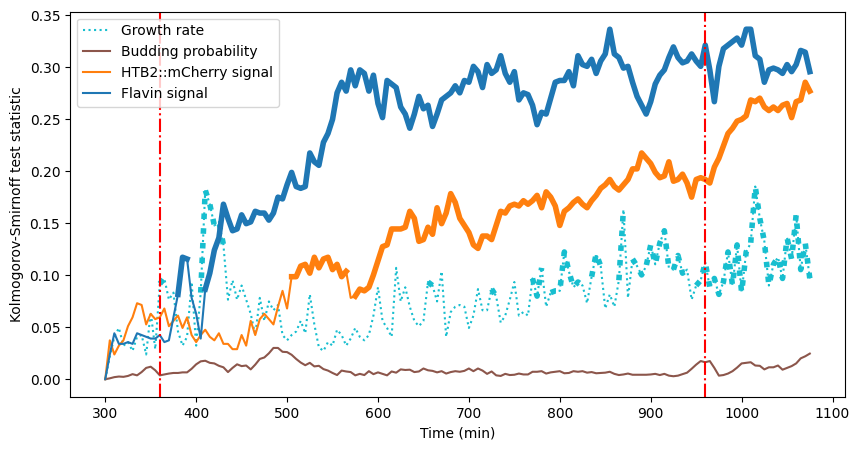
\includegraphics[width=\textwidth]{613_ks_highlight}
  \caption{
    Potassium-deficiency experiment.
    For each quantity, the Kolmogorov-Smirnov test statistics from two-tailed tests between the distribution at \SI{300}{\minute} and the distribution at each time point of interest is shown.
    The null hypothesis for each test is that the two samples are drawn from the same probability distribution, and thick lines indicate where the hypothesis is rejected ($p < 0.05$).
    Vertical lines (red) indicate changes in nutrient conditions.
  }
  \label{fig:biology-kdeficient-ks}
\end{figure}

% Conclusions are a bit iffy.  I probably need to think of new statistical tests.
As for the glucose-starvation experiment, I then investigated how the distribution of growth rates, budding probability, raw HTB2::mCherry intensity, and raw flavin intensity changes over the course of the experiment (figures~\ref{fig:biology-kdeficient-distribs},~\ref{fig:biology-kdeficient-ks}), using the \SI{300}{\minute} time point as the pre-potassium-deficiency reference point.
In contrast to the glucose-starvation experiment, the distribution of budding probability never showed a significant change from the pre-deficiency reference point throughout the experiment.
Additionally, the growth rates changed distribution profile when the growth rates dropped in the initial response to potassium depletion, and again later in the potassium-deficient condition.
Interestingly, the distribution of HTB2::mCherry intensities become more spread towards the end of the experiment, while the mean value of flavin intensity did not change as drastically at it did for the glucose-starvation experiment.

Taken together, my results suggest that even though there is an initial response to potassium depletion, cells resume growth, division, and generation of metabolic cycles soon after.
Although the chemostat study suggests that metabolic cycles should not occur when potassium is depleted, I observe metabolic cycles in single-cell conditions, though at a longer period and with less robustness.
My observations thus also show that the metabolic cycle is robust --- in other words, I showed that they still occur in a drastically changed nutrient condition.
However, my observations also warrant a model to reconcile the apparent differences between the chemostat and single-cell investigations.


%\section[Deletion strains]{Do single-cell flavin traces recapitulate dissolved-oxygen YMCs in chemostats? -- deletion strains}
\section{Metabolic cycles in deletion strains}
\label{sec:biology-deletions}

% \item swe1$\Delta$: gene responsible for CDC processes (another biological rhythm) e.g. DNA repair.  Deletion shown to affect CDC-YMC coupling.
% \item rim11$\Delta$: gene involved in circadian rhythm (another biological rhythm).  Deletion strain shown to have shorter YMCs.

To continue the investigation of whether single-cell flavin-based metabolic cycles recapitulate dissolved-oxygen metabolic cycles, I investigate the zwf1$\Delta$ and tsa1$\Delta$ tsa2$\Delta$ deletion strains.
With deletion strains, I can give some mechanistic insight on YMC, otherwise largely unknown.

Chemostat-based studies suggest that in the zwf1$\Delta$ strain, metabolic cycles are abolished but with little change in growth rate \parencite{tuCyclicChangesMetabolic2007}.
They interpret that entry into the pentose phosphate pathway, and thus production of NADPH, is required for the metabolic cycle.
\textit{ZWF1} codes for glucose-6-phosphate dehydrogenase, a key metabolic enzyme in the pentose phosphate pathway that plays a role in production of NADPH, which is a key player in YMC.
% ELABORATE MORE -- TAKE FROM ZWF1 ORG NOTE
Though, it is important to note that ALD6 and IDP2 can compensate this NADPH production \parencite{minardSourcesNADPHYeast2005}.


% TODO: Add single time series??  I've shown them for all the experiments so far, I just realised.
\begin{figure}
  \centering
  \begin{subfigure}[t]{0.45\textwidth}
   \centering
   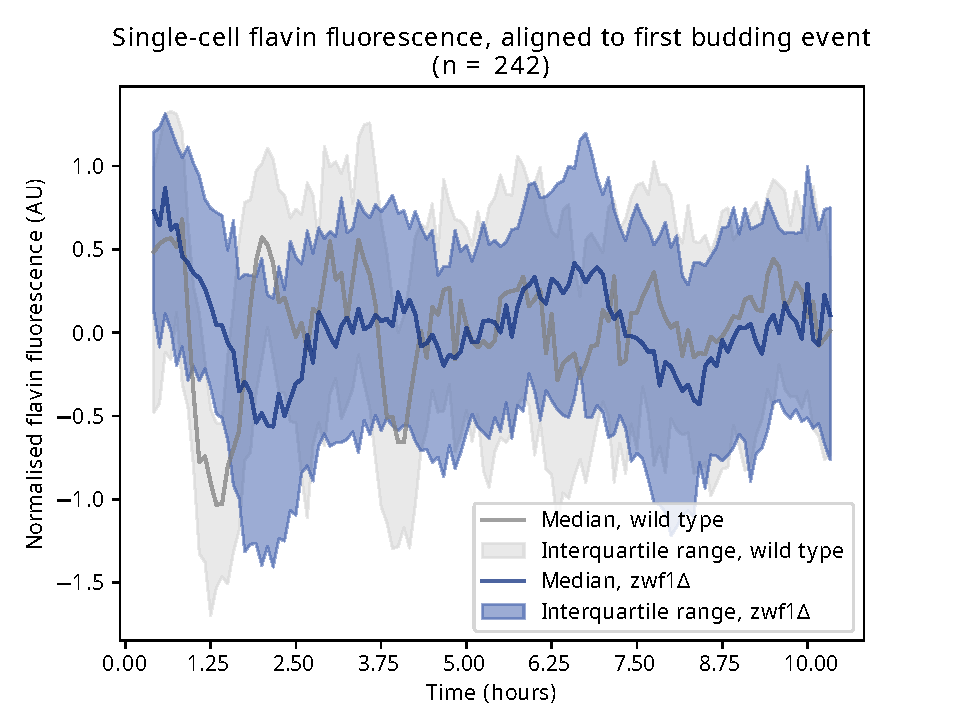
\includegraphics[width=\textwidth]{zwf1egf_409_6.pdf}
   \caption{
     Median flavin fluorescence signal across cells,%; each data point is the median of flavin fluorescence at each time point relative to the first birth.
     suggesting that flavin oscillations have some degree of synchrony with the cell division cycle, and oscillate at a period of approximately \SI{3}{\hour}.
   }
   \label{fig:biology-zwf1-median}
  \end{subfigure}%
  \begin{subfigure}[t]{0.45\textwidth}
   \centering
   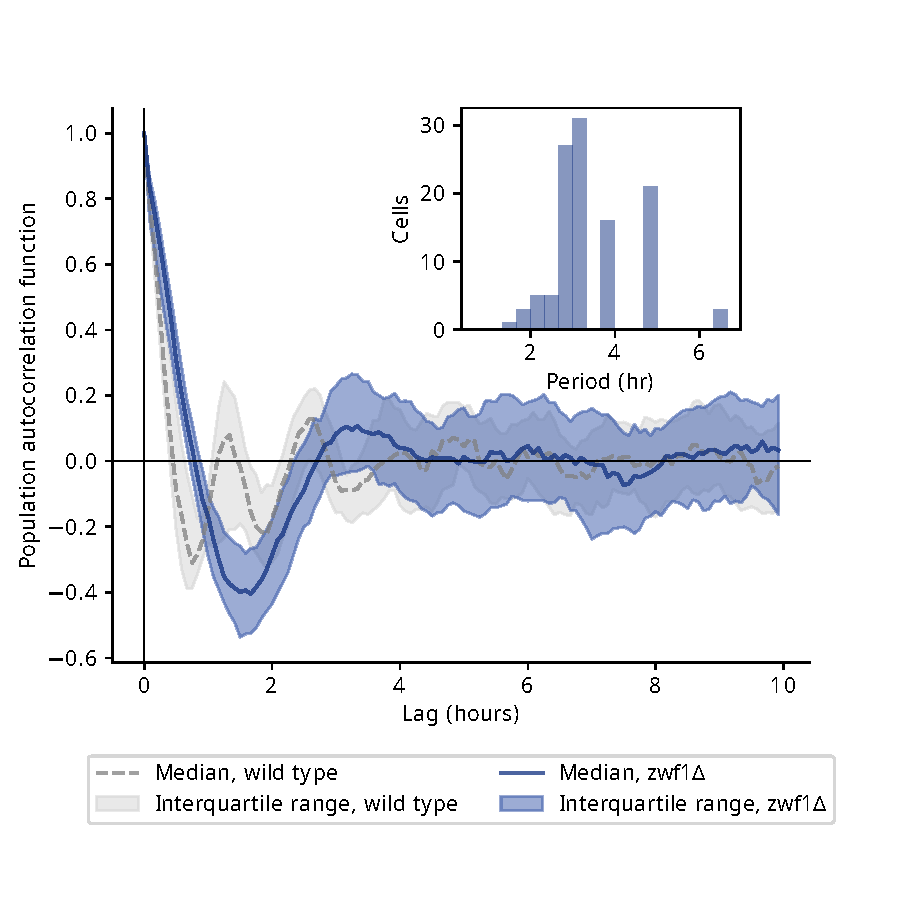
\includegraphics[width=\textwidth]{zwf1egf_409_12.pdf}
   \caption{
    Autocorrelation function of flavin fluorescence across cells, suggesting an average oscillation of approximately \SI{3}{\hour}, but with low robustness.
   }
   \label{fig:biology-zwf1-median}
  \end{subfigure}

  \begin{subfigure}[t]{0.45\textwidth}
   \centering
   \includegraphics[width=\textwidth]{zwf1egf_409_10.pdf}
   \caption{
    Distribution of signal-to-noise ratios computed for each flavin time series derived from zwf1$\Delta$ cells, showing a wide distribution of oscillation quality.
   }
   \label{fig:biology-zwf1-snr}
  \end{subfigure}%

  \caption{
    zwf1$\Delta$ (BY4741) cells in \SI{10}{\gram~\litre^{-1}} glucose generate metabolic oscillations.
  }
  \label{fig:biology-zwf1}
\end{figure}


To investigate the behaviour of zwf1$\Delta$ in single-cell microfluidics, I used a zwf1$\Delta$ strain with the BY4741 background.
Cells were pre-cultured in \SI{20}{\gram~\litre^{-1}} pyruvate over \SI{48}{\hour} and then cultured in \SI{10}{\gram~\litre^{-1}} glucose in the microfluidic device --- higher glucose concentrations disfavour growth in this strain.
As the strain had an auxotrophic background, the required nutrient supplements were also added.
Figure~\ref{fig:biology-zwf1} shows that while the reference BY4741 strain showed robust flavin oscillations of approximately \SI{1.5}{\hour}, the zwf$\Delta$ showed oscillations of approximately \SI{3}{\hour}, but with low robustness and a wide distribution of signal-to-noise ratios.
These result conflict with the results from the chemostat-based study that suggests that metabolic cycles are abolished in this strain.

Chemostat-based studies suggest that in the tsa1$\Delta$ tsa2$\Delta$ strain, metabolic cycles are shorter and exhibit an M-shaped dissolved oscillation trace due to an additional dip of oxygen consumption in the reductive-charging phase \parencite{caustonMetabolicCyclesYeast2015}. % TODO: Check with introduction.
The double deletion affects a pair of paralogous genes that are involved in redox metabolism (key player of metabolic cycle), linked to circadian rhythm (another biological rhythm), therefore it was targeted as a potentially important gene for the metabolic cycle.

\begin{figure}
  \centering
  \begin{subfigure}[t]{0.45\textwidth}
   \centering
   \includegraphics[width=\textwidth]{tsa1tsa2morgan_1649_6.pdf}
   \caption{
     Median flavin fluorescence signal across cells,%; each data point is the median of flavin fluorescence at each time point relative to the first birth.
     suggesting that flavin oscillations has weak synchrony with the cell division cycle, and oscillate at a period of approximately \SI{3}{\hour}.
   }
   \label{fig:biology-tsa1tsa2-median}
  \end{subfigure}%
  \begin{subfigure}[t]{0.45\textwidth}
   \centering
   \includegraphics[width=\textwidth]{tsa1tsa2morgan_1649_12.pdf}
   \caption{
    Autocorrelation function of flavin fluorescence across cells, showing a lack of oscillations at a regular frequency across the population, in contrast to more regular oscillations in the wild type.
   }
   \label{fig:biology-tsa1tsa2-median}
  \end{subfigure}

  \begin{subfigure}[t]{0.45\textwidth}
   \centering
   \includegraphics[width=\textwidth]{tsa1tsa2morgan_1649_10.pdf}
   \caption{
    Distribution of signal-to-noise ratios computed for each flavin time series derived from tsa1$\Delta$ tsa2$\Delta$ cells, showing that the quality of oscillations is comparable to growth in pyruvate.
   }
   \label{fig:biology-tsa1tsa2-snr}
  \end{subfigure}%

  \caption{
    tsa1$\Delta$ tsa2$\Delta$ (BY4742) cells in \SI{10}{\gram~\litre^{-1}} glucose do not robustly generate metabolic oscillations.
  }
  \label{fig:biology-tsa1tsa2}
\end{figure}


To investigate the behaviour of tsa1$\Delta$ tsa2$\Delta$ in single-cell microfluidics, I used a tsa1$\Delta$ tsa2$\Delta$ strain with the BY4742 background.
To be consistent with zwf1$\Delta$, cells were pre-cultured and cultured in the same conditions, but with the appropriate supplements for the auxotrophy of BY4742.
% Is this because of a wide variety of oscillation frequencies?  Look at the FFT inset, or do additional investigations.
Figure~\ref{fig:biology-tsa1tsa2} suggests that, despite relatively high-quality oscillations as evidenced by the signal-to-noise ratios, the autocorrelation function does not show oscillations at a regular frequency across the population.
Although, the median fluorescence signal and Fourier spectra suggest that a \SI{3}{\hour} oscillation is prominent in the population.
In short, single-cell metabolic oscillations are not reliably generated from the auxotrophic tsa1$\Delta$ tsa2$\Delta$ strain.
In addition, I also observe cells showing `sick' phenotypes (bloating and clogging) earlier in the experiment than the wild type.

Taken together, there are striking discrepancies between the metabolic cycle observed as dissolved oxygen oscillations from the chemostat and the metabolic cycle observed as flavin autofluorescence oscillations in single-cell conditions in the zwf1$\Delta$ and tsa1$\Delta$ tsa2$\Delta$ deletion strains.
These discrepancies may be partly explained by the lack of information about cell-to-cell heterogeneity in the chemostat.
Chemostat studies commonly state that they induce metabolic cycles by imposing glucose starvation in the culture for some time.
In light of the glucose-starvation results in section~\ref{sec:biology-abrupt}, these metabolic cycles may be the combined effect of individual cells' response to starvation.
A lack of dissolved oxygen oscillations in zwf1$\Delta$ with a growth rate similar to wild-type \parencite{tuCyclicChangesMetabolic2007} may be explained by a loss of ability to reset the phase of the metabolic cycle or a variety of metabolic cycle lengths.
In addition, the M-shaped dissolved oxygen oscillations in tsa1$\Delta$ tsa2$\Delta$ may be explained by the combined effect of sub-populations that have different metabolic cycle periods.
These ideas are additionally supported by how my metabolic cycles are far shorter than the periods of chemostat-based metabolic cycles.

\section{Discussion}
\label{sec:biology-discussion}

\subsection{Interpretation of results}
\label{subsec:biology-discussion-interpretation}

% TODO:
% - Check whether this recapitulates the hypothesis/aims I presented at the beginning of the chapter.
% - Check how repetitive this is with the main part of the chapter, and kill stuff accordingly.
% - Read the main part as I've come up with some re-interpretations.  The interpretation here must take these into account and also sum them up concisely.

This chapter confirms the presence of flavin-based single-cell metabolic cycles, which are autonomous and gate the cell division cycle.
Consistent with previous single-cell microfluidics studies, in high glucose, flavin cycles are asynchronous between cells and peaks in flavin fluorescence coincide with bud formation.
Results in pyruvate reveal that as the metabolic cycle lengthens, G1 lengthens but S/M stays the same length, reinforcing a model in which a specific phase of the metabolic cycle gates entry into the cell division cycle.
%This is consistent with \textcite{oneillEukaryoticCellBiology2020} and (add other citations here).
Cross-correlation between flavin and mCherry signals further confirm the sequence of events while the two biological oscillations (metabolic cycle and cell division cycle) progress.
This relationship is particularly obvious in pyruvate.
Specifically, when the new bud forms, the mother cell's flavin fluorescence peaks.
Subsequently, the cell synthesises new histones in S phase, then the cell enters anaphase --- characterised by the sharp drop in the mCherry signal --- as the flavin fluorescence is at its trough.
Importantly, metabolic cycles still occur even when cells do not divide.
This holds true for `one-off' skipping of cell division and conditions in which cells pause cell division for long periods of time.

This chapter additionally shows that cells individually generate metabolic cycles and individually adapt them in response to nutrient changes.
The literature disputes whether metabolic oscillations arise from interactions between cells or whether cells individually generate oscillations.
In my observations, even though the cells are physically separated in traps and nutrient media flows through them, single-cell flavin oscillations can synchronise and reset phase in certain conditions.
Diffusible metabolites cannot be responsible.
I thus conclude that each cell --- on its own --- can reset its metabolic cycle in response to nutrient changes.
This conclusion does not mean that cells \emph{cannot} communicate with each other, but communication is \emph{not required}.

Observations of the two oscillators during starvation piques curiosity about their mechanistic basis in such conditions.
% TODO: Come up with new analysis to prove/disprove this.  Or link this with existing results.  It's still quite unclear to me.
For the cell division cycle, the most likely explanation is if starvation occurs before START, cell remain in pause; if starvation occurs after START, cells go into pause.
In contrast, the biochemical mechanism that the cell uses to reset the phase of its metabolic cycle, is unclear, and it owes to the poor characterisation of the biochemistry of the metabolic cycle in general.

This chapter confirms that cells adapt their metabolic cycle to nutrient conditions.
Namely, the behaviour of the metabolic cycle changes when the cells are grown on low glucose or on pyruvate.
The biochemical interpretation could be that nutrient conditions that favour respiration over fermentation --- and thus slower growth rate --- leads to slower YMCs.
% Do the periods conform to those reported by \textcite{papagiannakisAutonomousMetabolicOscillations2017}?  If not, why?

This chapter also attempts to reconcile chemostat and single-cell studies.
In chemostats, glucose is limiting \parencite{jonesCyberneticModelGrowth1999}.
Synchrony of metabolic cycles between cells in respiring conditions may explain observations in chemostat as cells are near glucose starvation in these conditions.

Single-cell metabolic cycles in zwf1$\Delta$ are inconsistent, and this may explain the absence of dissolved-oxygen oscillations in the chemostat.
zwf1$\Delta$ affects many metabolic processes; most notably, it removes a major pathway of NAD(P)H generation from reduction of NAD(P)\textsuperscript{+}.
The most abundant flavoproteins involve NAD(P)H redox, so it is reasonable to believe that flavin oscillations are affected.
Perhaps zwf1$\Delta$ impairs the metabolic cycle in some way.
A similar logic likely applies to tsa1$\Delta$ tsa2$\Delta$ --- perhaps the interaction between a more variable length of metabolic oscillations interacts with population synchrony, or lack thereof, in the chemostat.
Furthermore, the tsa1$\Delta$ tsa2$\Delta$ double deletion affects the peroxiredoxin-thioredoxin system, therefore affecting redox balance, likely in an extensive way.

The fact that metabolic oscillations are present when the medium is potassium-free can be seen as more evidence that there is no straight one-to-one correspondence between dissolved-oxygen metabolic oscillations in the chemostat and single-cell flavin oscillations from single cells.
Therefore, the difference between single-cell and chemostat traces warrant a model to explain the differences, likely involving subpopulations.
My observations thus also highlight a weakness of chemostat experiments.


\subsection{Study caveats and future directions}
\label{subsec:biology-discussion-caveats}

% Worth reading with the introduction to iron out any logical inconsistencies.

\subsubsection{Characteristics of the single-cell metabolic cycle}
\label{subsec:biology-discussion-caveats-characteristics}

Time series of NAD(P)H oscillations, especially if recorded alongside flavin in the same cells, would strengthen the evidence that the flavin autofluorescence oscillations in this chapter are equivalent to the single-cell metabolic oscillations described by previous microfluidics studies.
However, due to technical limitations of the fluorescence microscope and image acquisition set-up, I have not been able to acquire such data.
If I have time series of NAD(P)H oscillations, I would compare the timing of its peaks with that of flavin and budding events to make sure that the sequence of events is consistent with \textcite{papagiannakisAutonomousMetabolicOscillations2017} and \textcite{baumgartnerFlavinbasedMetabolicCycles2018}.
Such data would also provide a novelty: two fluorophores that act as read-outs of the metabolic cycle have, to my knowledge, never been recorded from the same cell.

To explore the link between the components of the flavin signal of the cell and cycling of lipid stores as a proposed biochemical mechanism of the metabolic cycle, the fas1$\Delta$ strain may be studied.
This is a good candidate because \textit{FAS1} codes for the most abundant flavoprotein, the beta subunit of fatty acid synthetase, which happens to have a role in lipid metabolism.
The investigation may be complemented with a rescue experiment using lipid sources such as glycerol trihexanoate or glycerol trioctanoate.
This avenue of exploration may lead to additional insight to the biochemical basis of the yeast metabolic cycle, which is still poorly characterised.

To explore the conditions that make budding yeast cells reset their metabolic cycle phases, future experiments may include adding carbon sources in bulk, using the media-switching system of ALCATRAS.
Such experiments could include acetate, acetaldehyde, or ethanol \parencite{kuangMsn2RegulateExpression2017, krishnaMinimalPushPull2018}.
Insights from such experiments can be combined with that of the glucose-starvation experiment and may lead to a broader understanding of the control of the sequence of events in the metabolic cycle.

\subsubsection{Chemostat vs single-cell}
\label{subsec:biology-discussion-caveats-chemostat}

Further work can be done to address the discrepancies between the chemostat and single-cell microfluidics.
Such work includes analysing sub-populations, additional nutrient conditions, or using different experimental hardwire entirely.

Sub-populations that produce metabolic cycles of different properties likely explain the discrepancy between the chemostat and single-cell microfluidics.
This model is likely for the zwf1$\Delta$ strain: the large spread of signal-to-noise ratios suggest that there can be a group of cells that produce noisy, low-amplitude metabolic cycles and another group that produce higher-quality and more robust metabolic cycles.
In such a case, the time series featurisation and clustering as discussed on the previous chapter may be useful in defining subpopulations, especially with the large datasets I handle,
% There are methods that don't rely on machine learning -- consult notes with Andrew Millar

Low glucose conditions emulate the environmental conditions in the chemostat and may lead to long metabolic cycles, thus explaining why cycles with periods up to \SI{14}{\hour} have been observed.
However, the glucose concentrations in chemostats are below the tolerance of measurement with current technologies, therefore the limiting concentration of \SI{10}{\milli\gram~\litre^{-1}} used in this chapter can be used.
Experiments with deletion strains can then be performed under these low-glucose conditions to investigate whether such conditions lead to a closer equivalence between chemostat and single-cell studies, thus explaining the results from chemostat-based studies of the deletion strains.

% Fact-check this!
Additionally, feast-and-famine conditions have been modelled \parencite{jonesCyberneticModelGrowth1999} and observed \parencite{oneillEukaryoticCellBiology2020} in chemostat cultivation of yeast.
Further experiments can therefore take advantage of the rapid media-switching capabilities of ALCATRAS, and include regular glucose pulsing: cells are fed with a glucose-limited medium for an amount of time, then switched on to the glucose-rich medium for \SI{10}{\minute}, and the cycle repeats.
The interval between glucose pulses can be varied to investigate the effect of an external entraining mechanism on the system of coupled oscillators that defines the yeast metabolic cycle.
This design would be similar to \textcite{charvinForcedPeriodicExpression2009}, which investigated the effect of intervals of glucose pulsing on the cell division and circadian cycles in budding yeast.
A glucose pulsing experiment can thus also lead to an interesting mathematical modelling study.

Finally, a turbidostat can be a middle-ground between chemostat and single-cell experiments and can be used to explore the chemostat-single cell discrepancy.
Turbidostat experiments were not performed due to a lack of hardware and expertise in the research group.
